\documentclass[11pt]{report}

% For including image file
\usepackage{graphicx, color}

% For including collection of image
%\usepackage{subcaption}

% For generating hyper links

% For coloring text
\usepackage{xcolor}

%\usepackage{hyperref}
\usepackage[linkbordercolor=white, colorlinks=true, urlcolor=black, linkcolor=black]{hyperref}

% Margin of the page
\usepackage[top=0.5in, bottom=1in, left=1in, right=1in]{geometry}

%For adding nomenclature
%\usepackage{nomencl}
%\makenomenclature
%\renewcommand{\nomname}{Annotation}

% For cover page tikz image 
%\usepackage{tikz}
%\usetikzlibrary{calc}

% For including a piece of code
%\usepackage{listings}

% Images folder
%\graphicspath{{Images/}}

\usepackage{titlesec}

\titleformat{\chapter}[display]
{\normalfont\Large\filcenter\sffamily}
{\vspace*{\fill}
 \titlerule[1pt]%
 \vspace{1pt}%
 \titlerule
 \vspace{1pc}%
 \LARGE\MakeUppercase{\chaptertitlename}~\thechapter}
{1pc}
{\titlerule\Huge}
[\vspace*{\fill}\newpage]

\titlespacing*{\chapter}{0pt}{0pt}{0pt}

\titleformat{name=\chapter,numberless}[display]
{\normalfont\Large\filcenter\sffamily}
{}
{0pt}
{\titlerule[1pt]\Huge}
[\titlerule]

\usepackage{pdfpages}

\begin{document}

\tableofcontents

\chapter{Lecture 1}
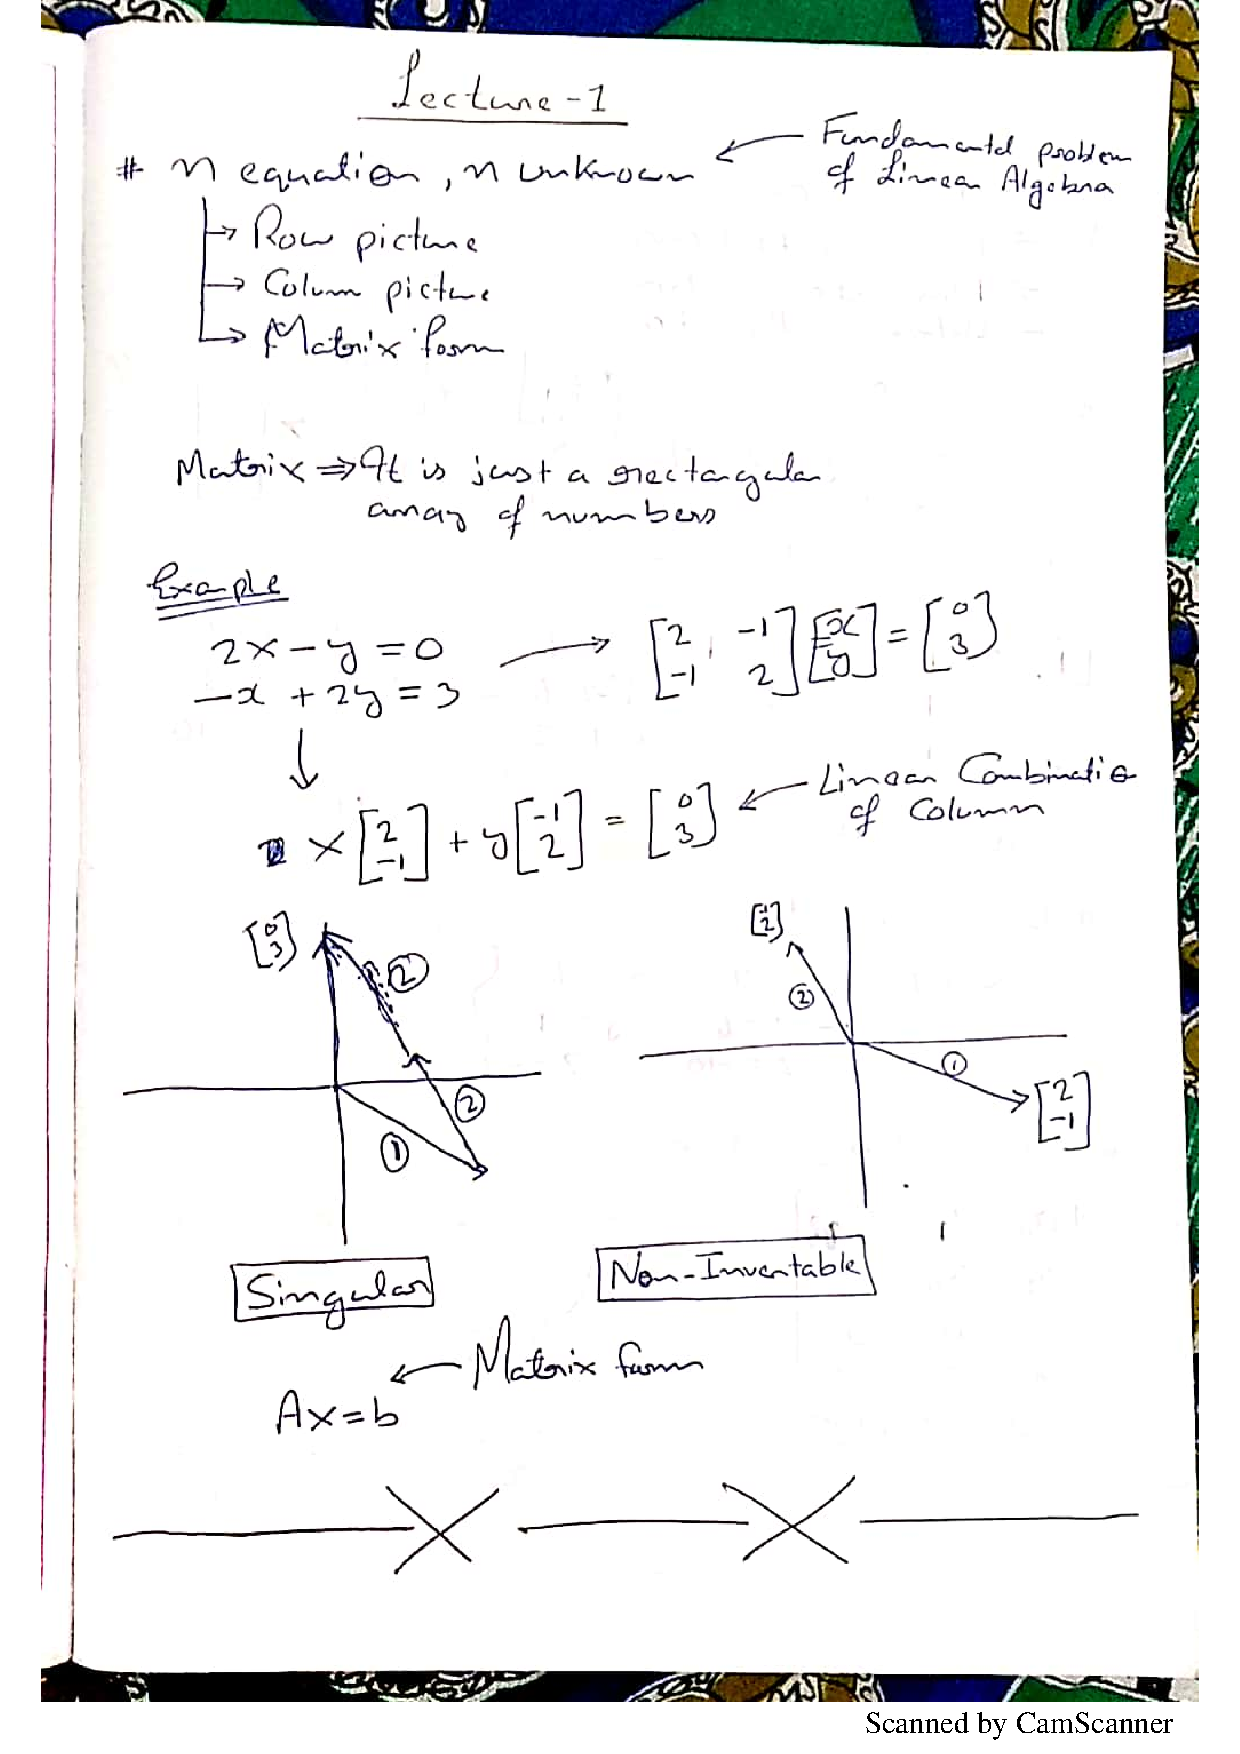
\includepdf[page=-]{./raw_files/1.pdf}

\chapter{Lecture 2}
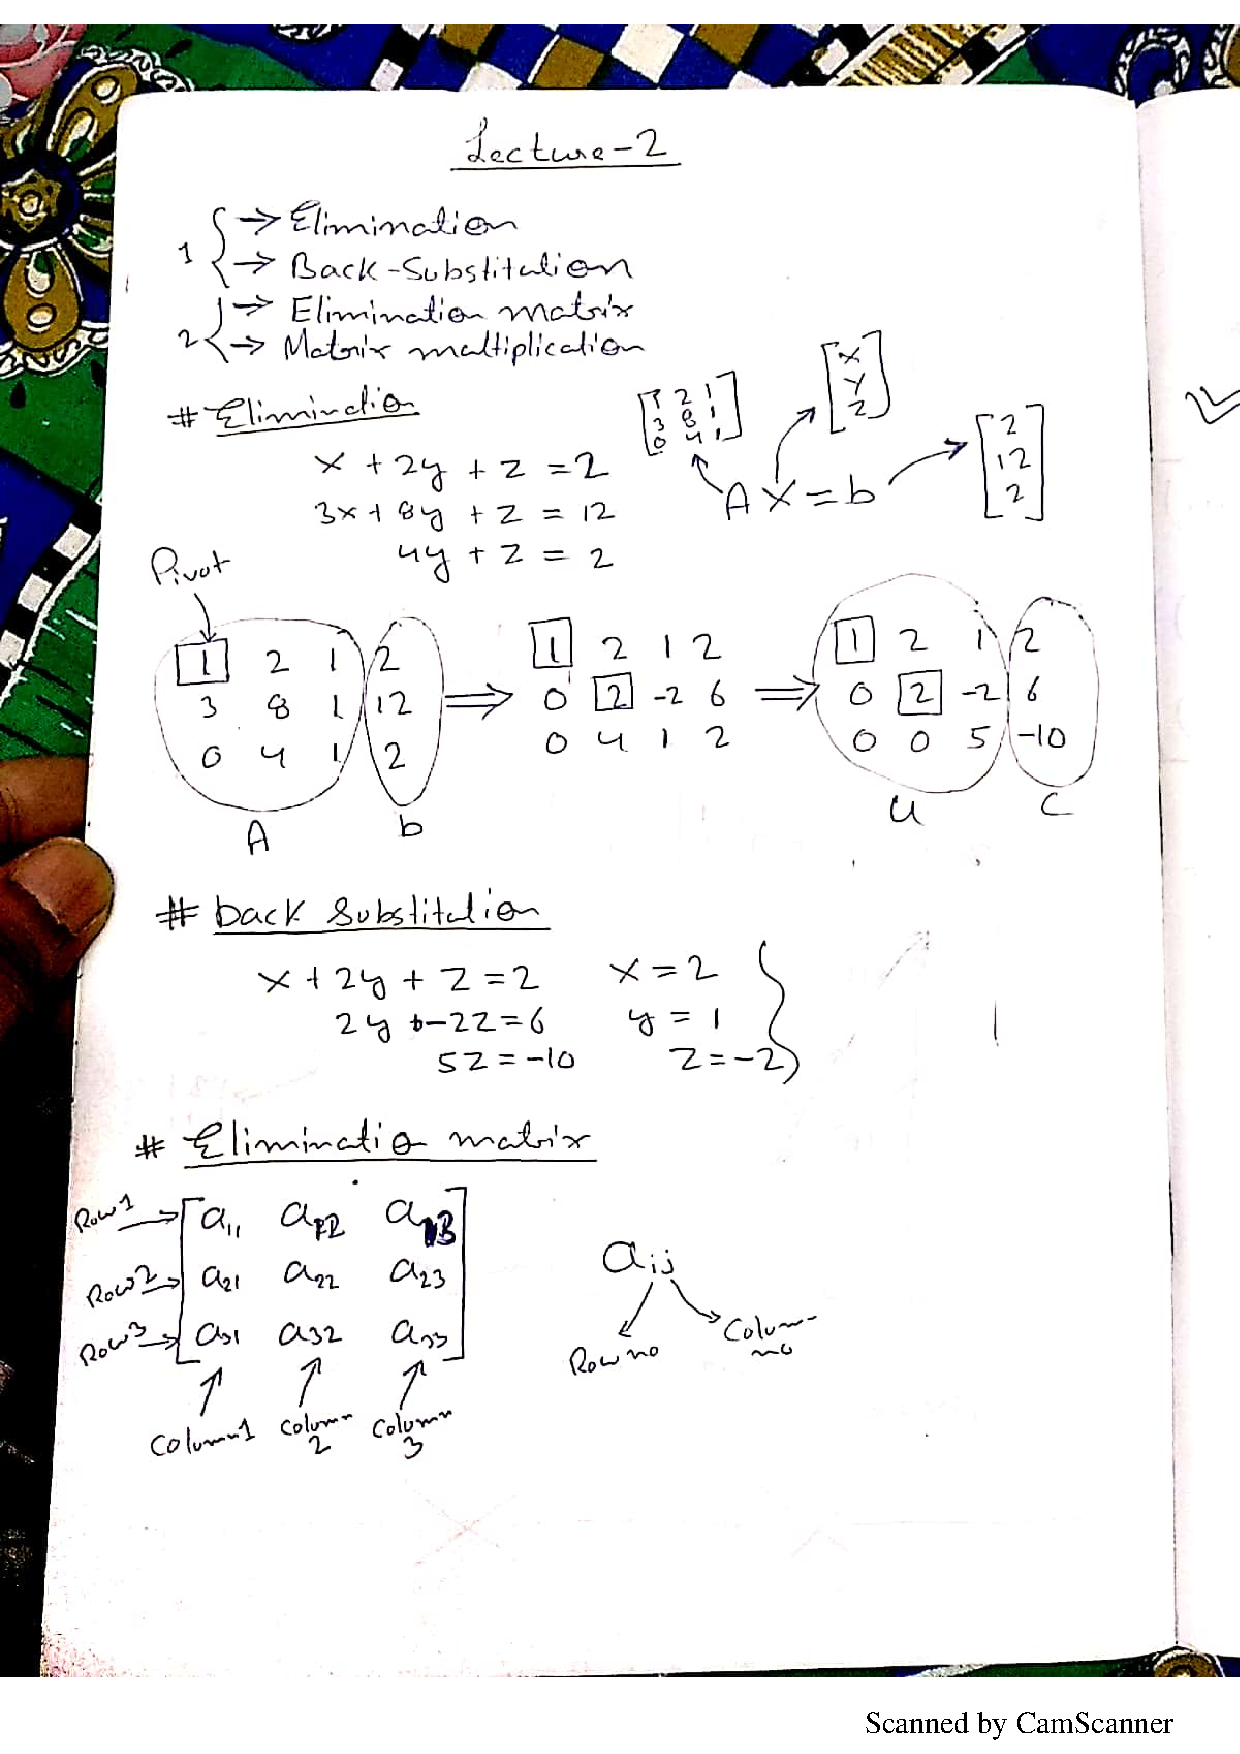
\includepdf[page=-]{./raw_files/2.pdf}

\chapter{Lecture 3}
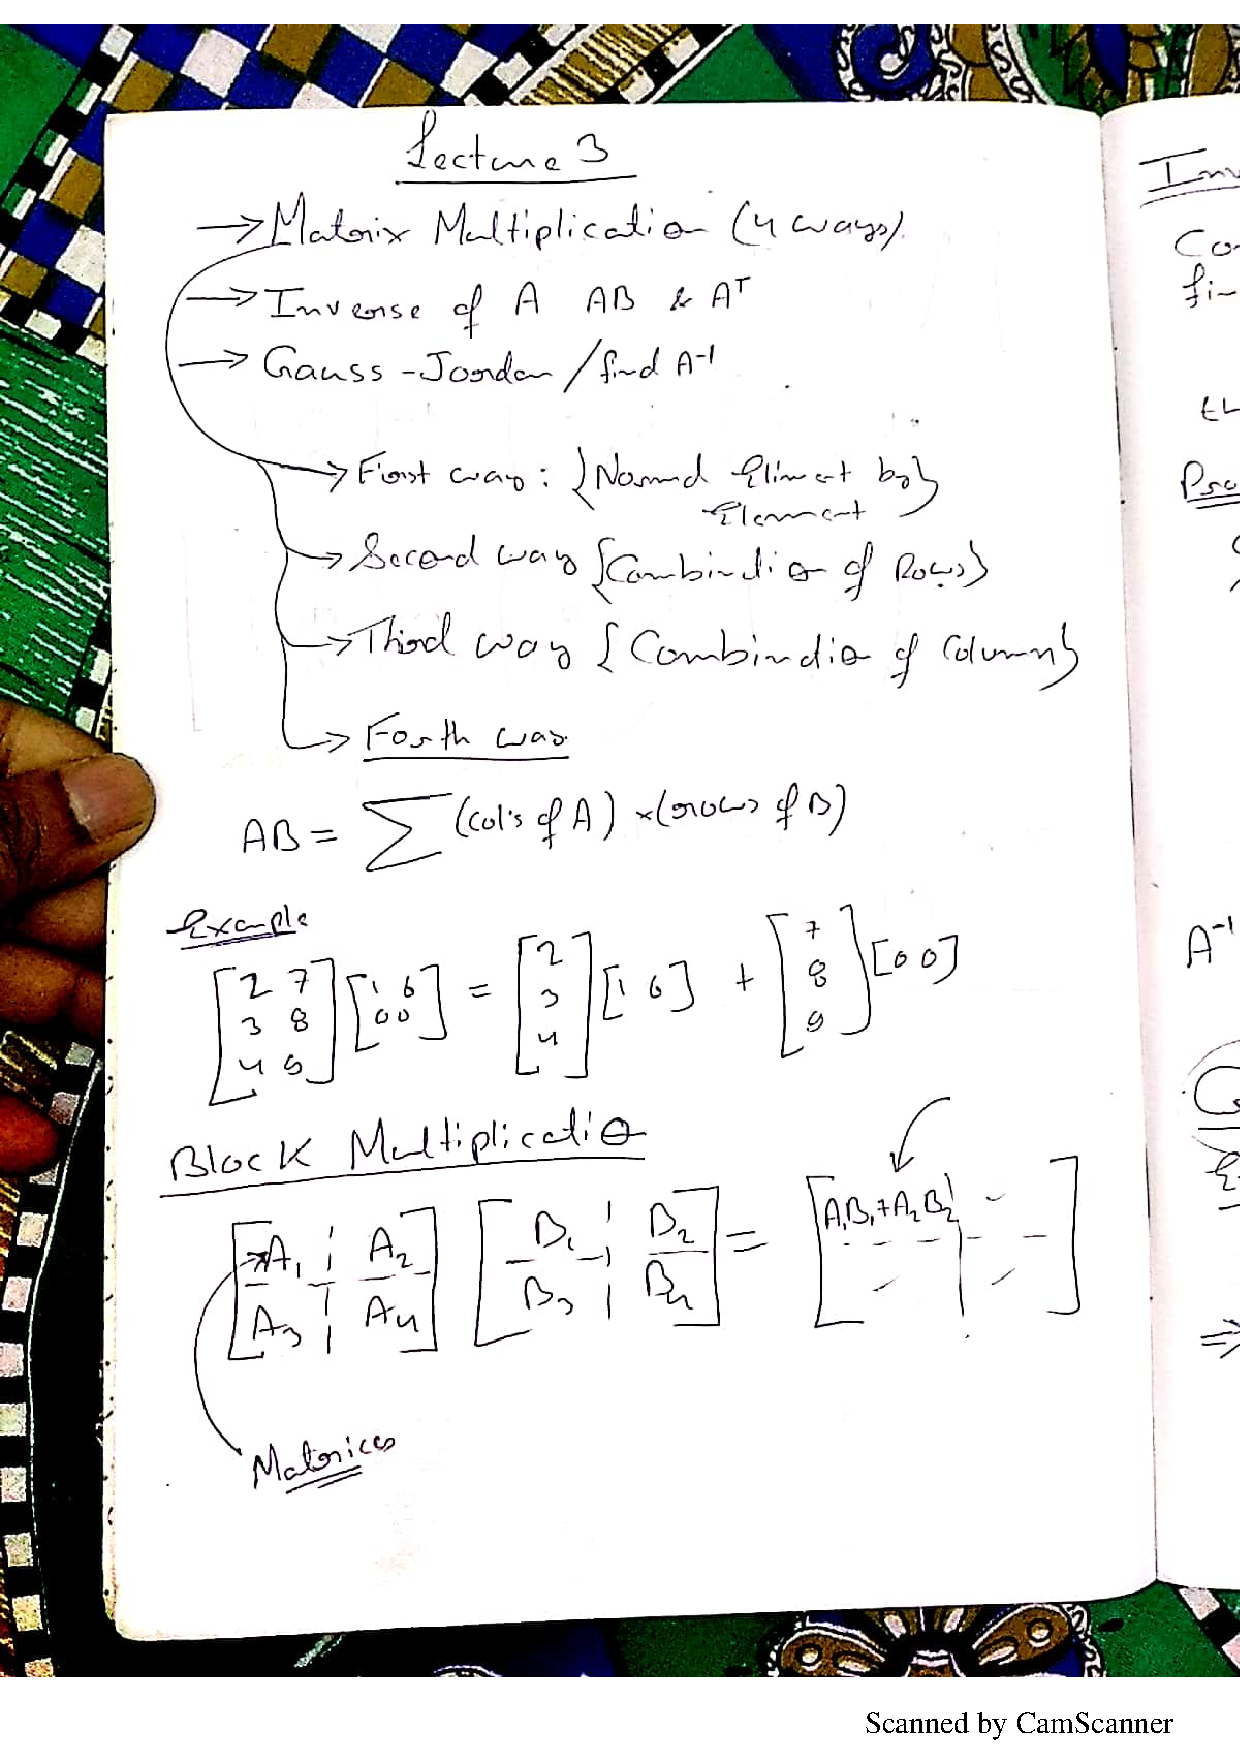
\includepdf[page=-]{./raw_files/3.pdf}

\chapter{Lecture 4}
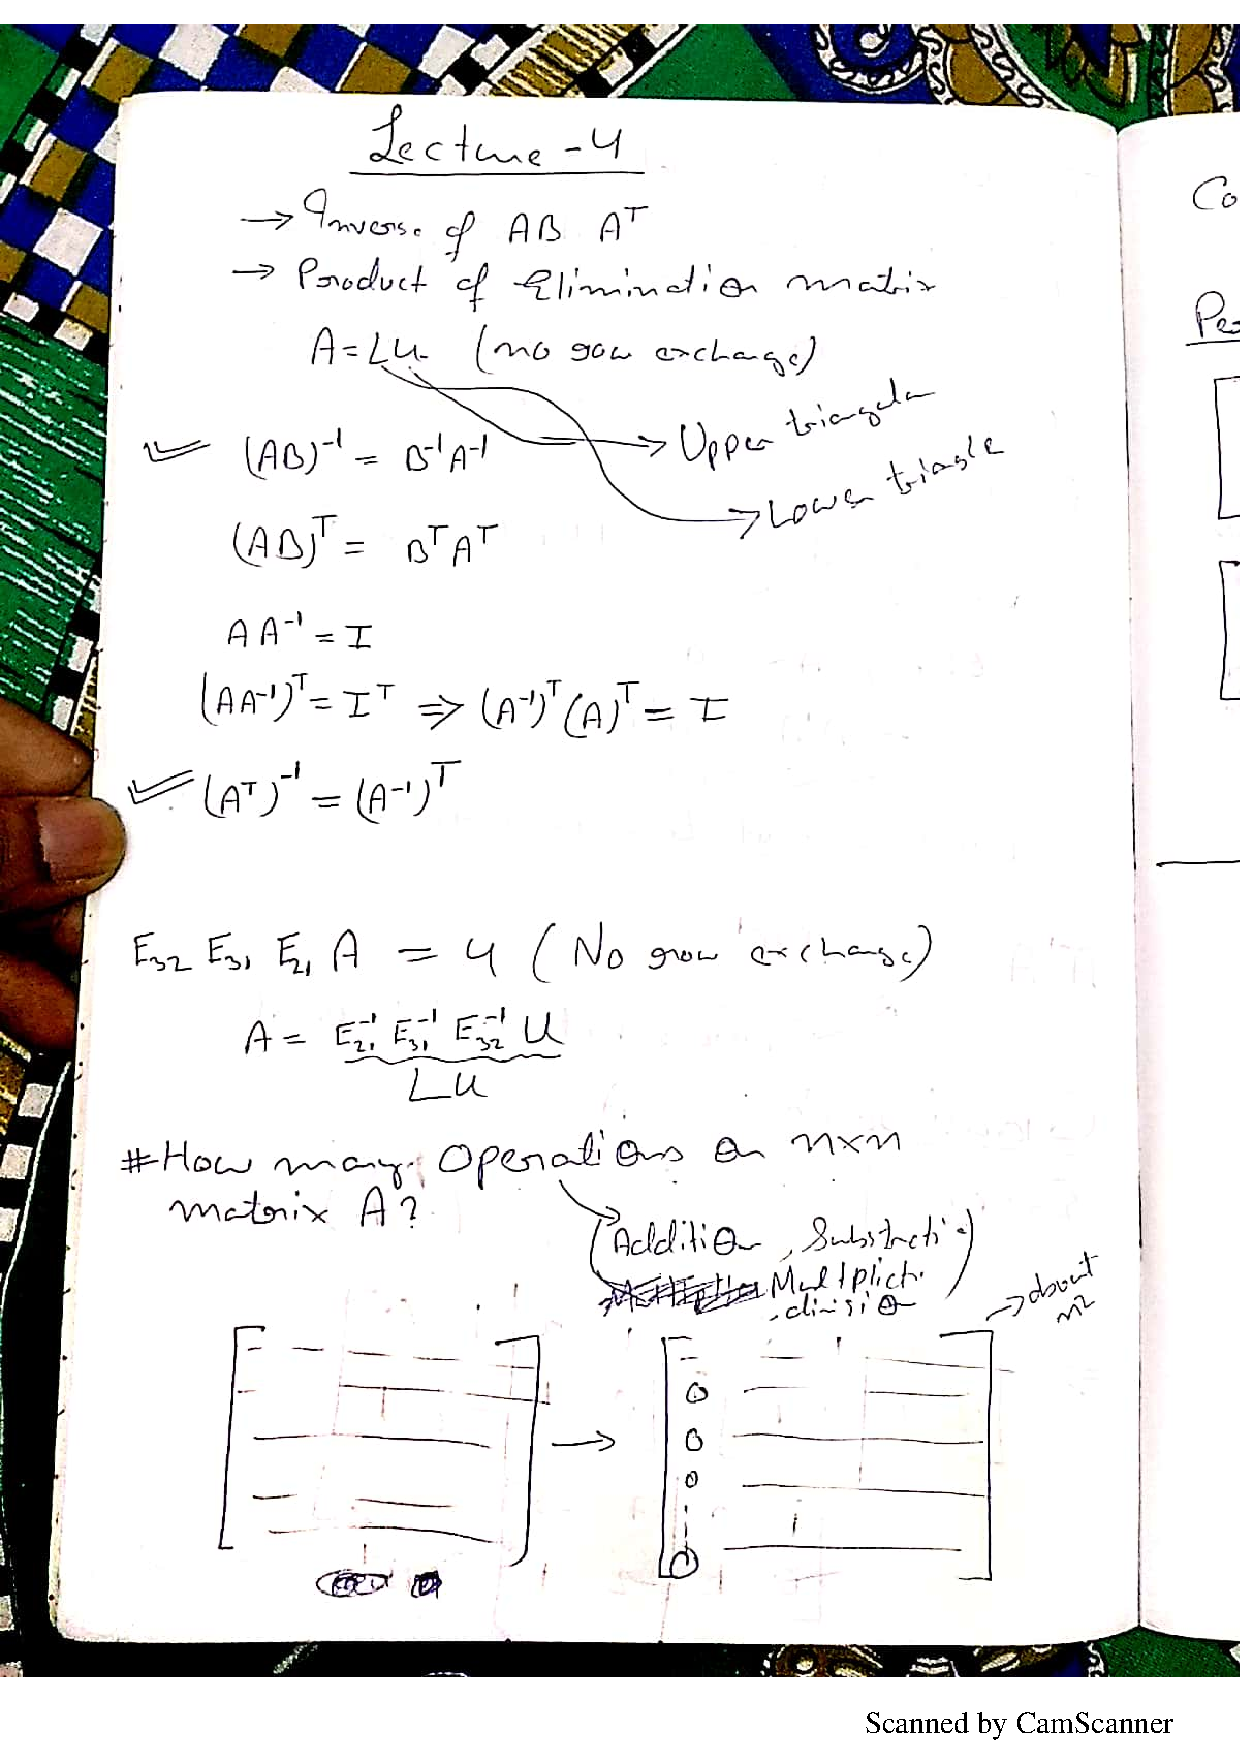
\includepdf[page=-]{./raw_files/4.pdf}

\chapter{Lecture 5}
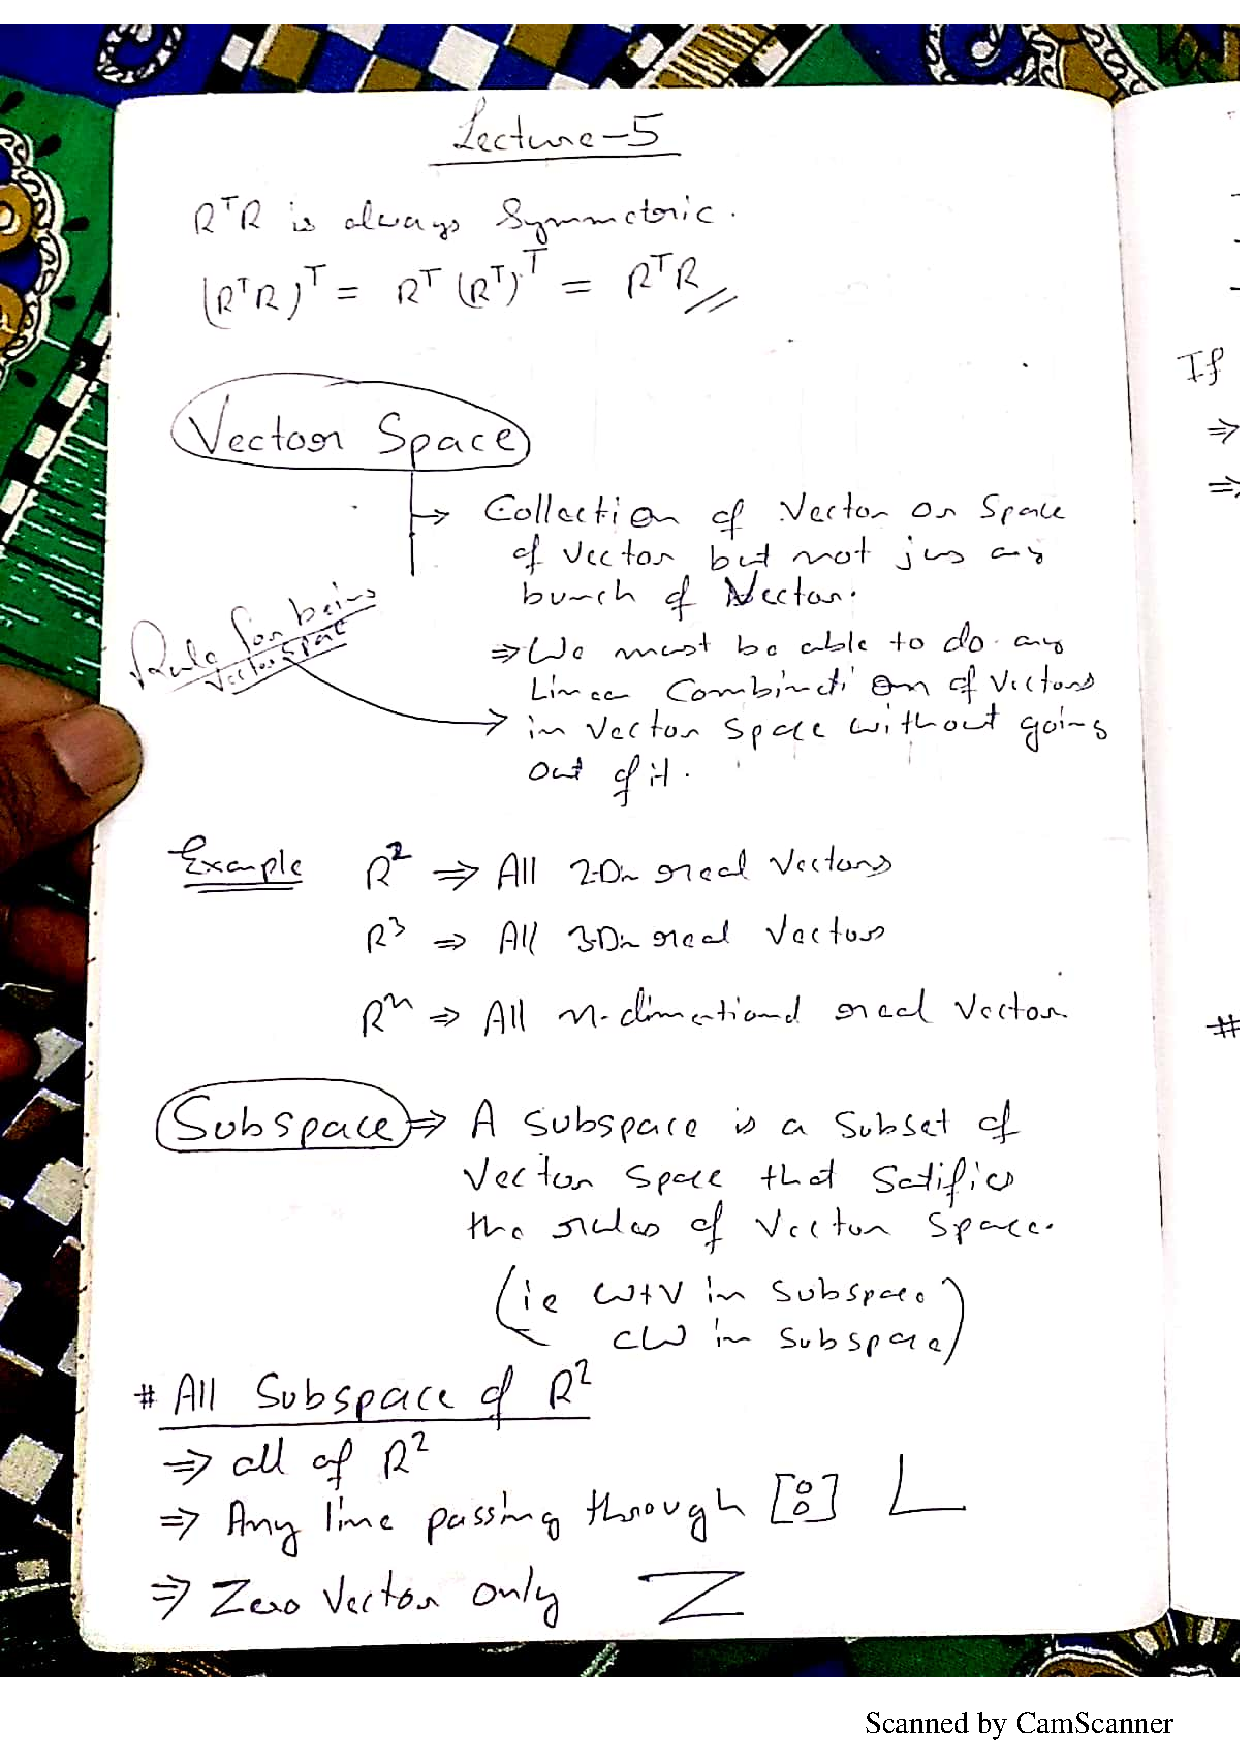
\includepdf[page=-]{./raw_files/5.pdf}

\chapter{Lecture 6}
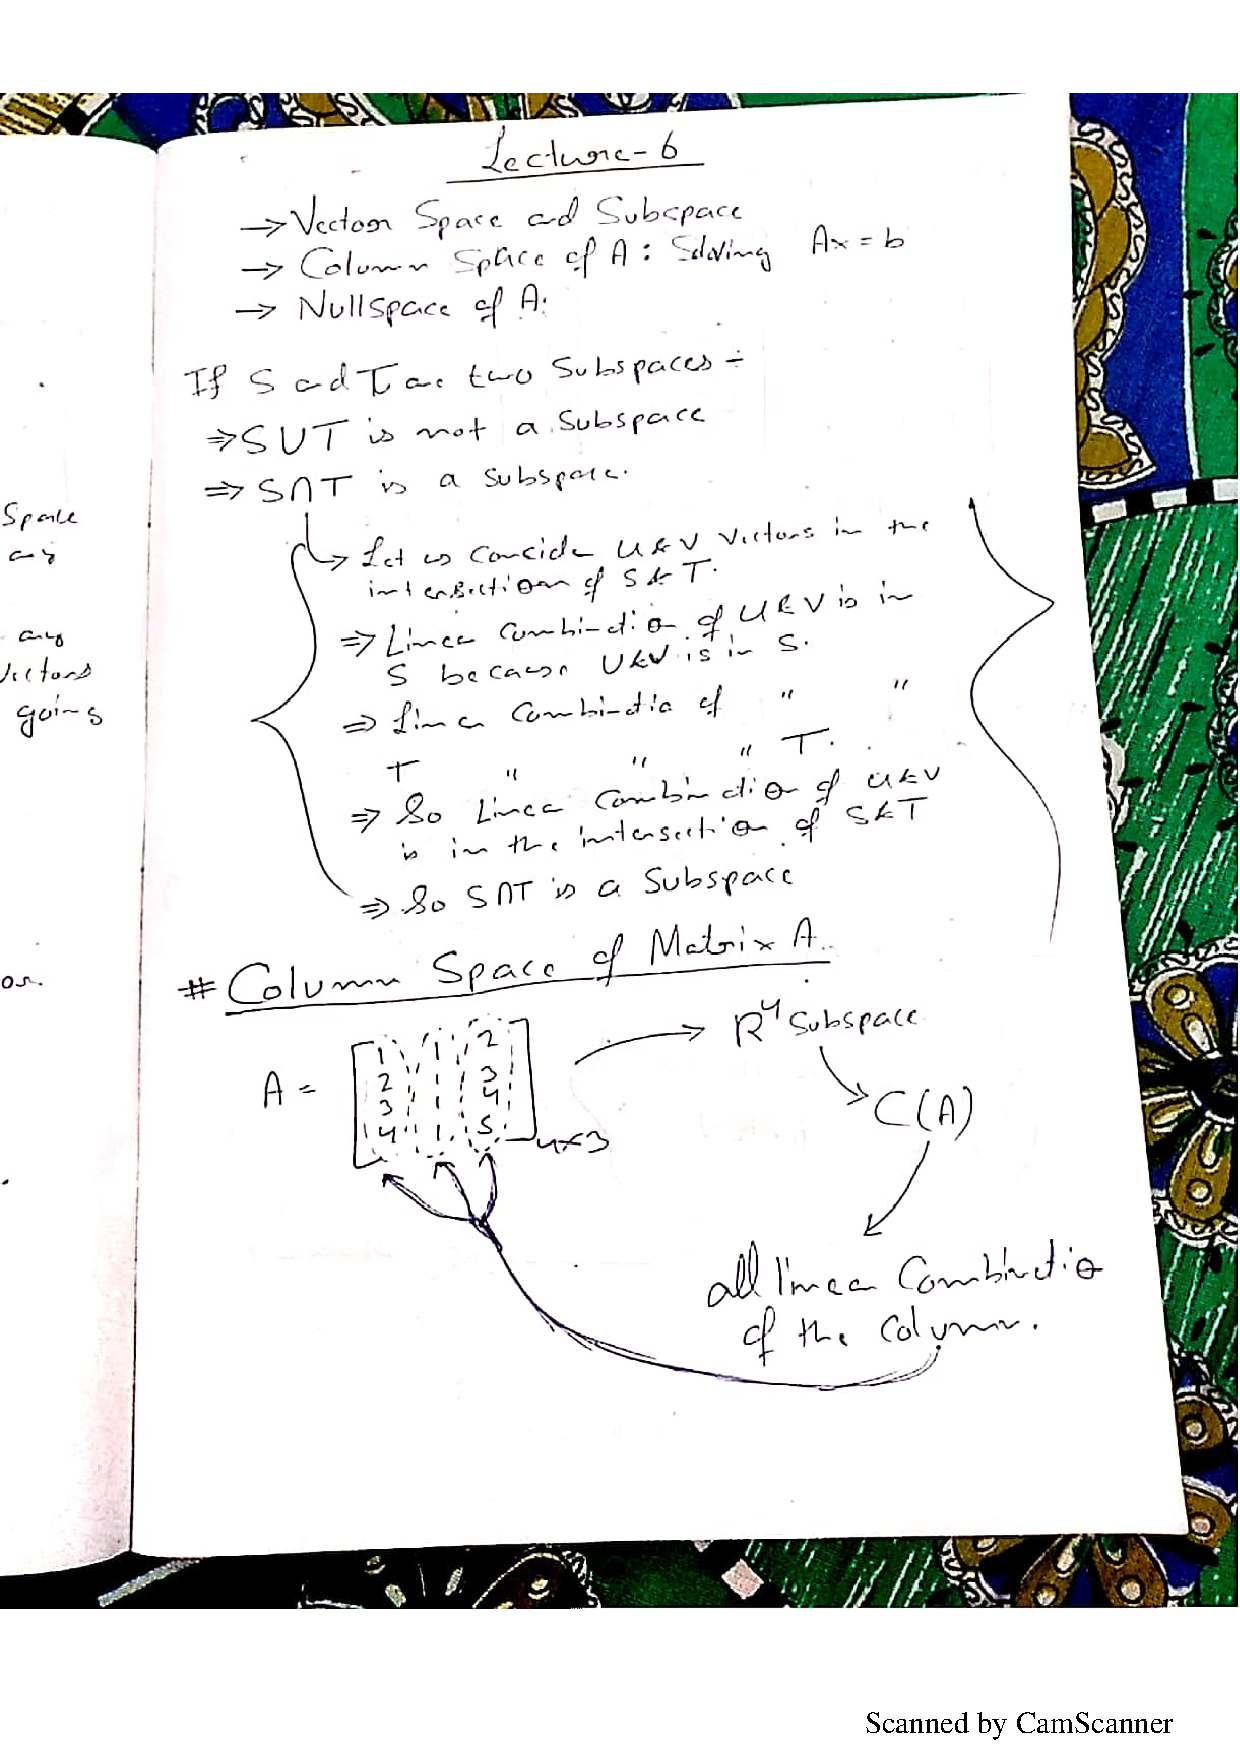
\includepdf[page=-]{./raw_files/6.pdf}

\chapter{Lecture 7}
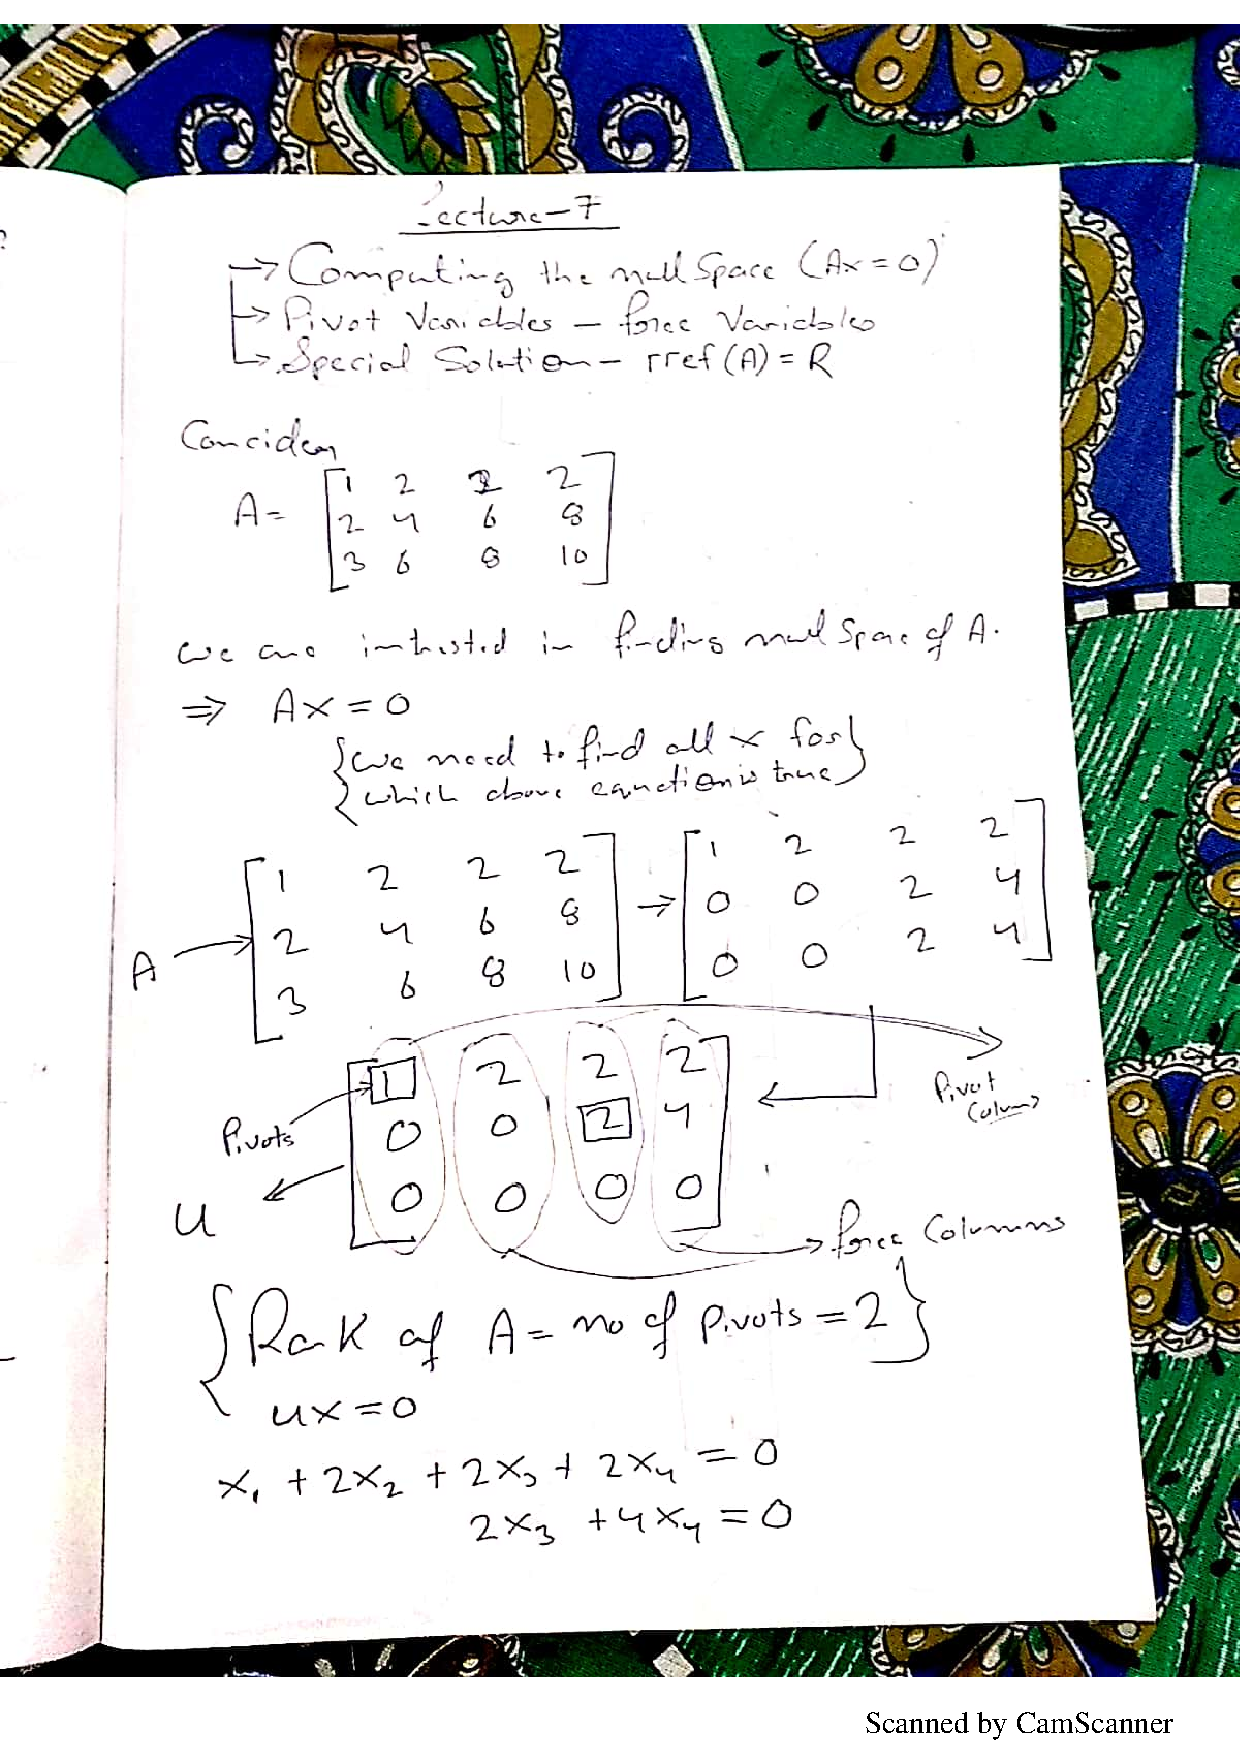
\includepdf[page=-]{./raw_files/7.pdf}

\chapter{Lecture 8}
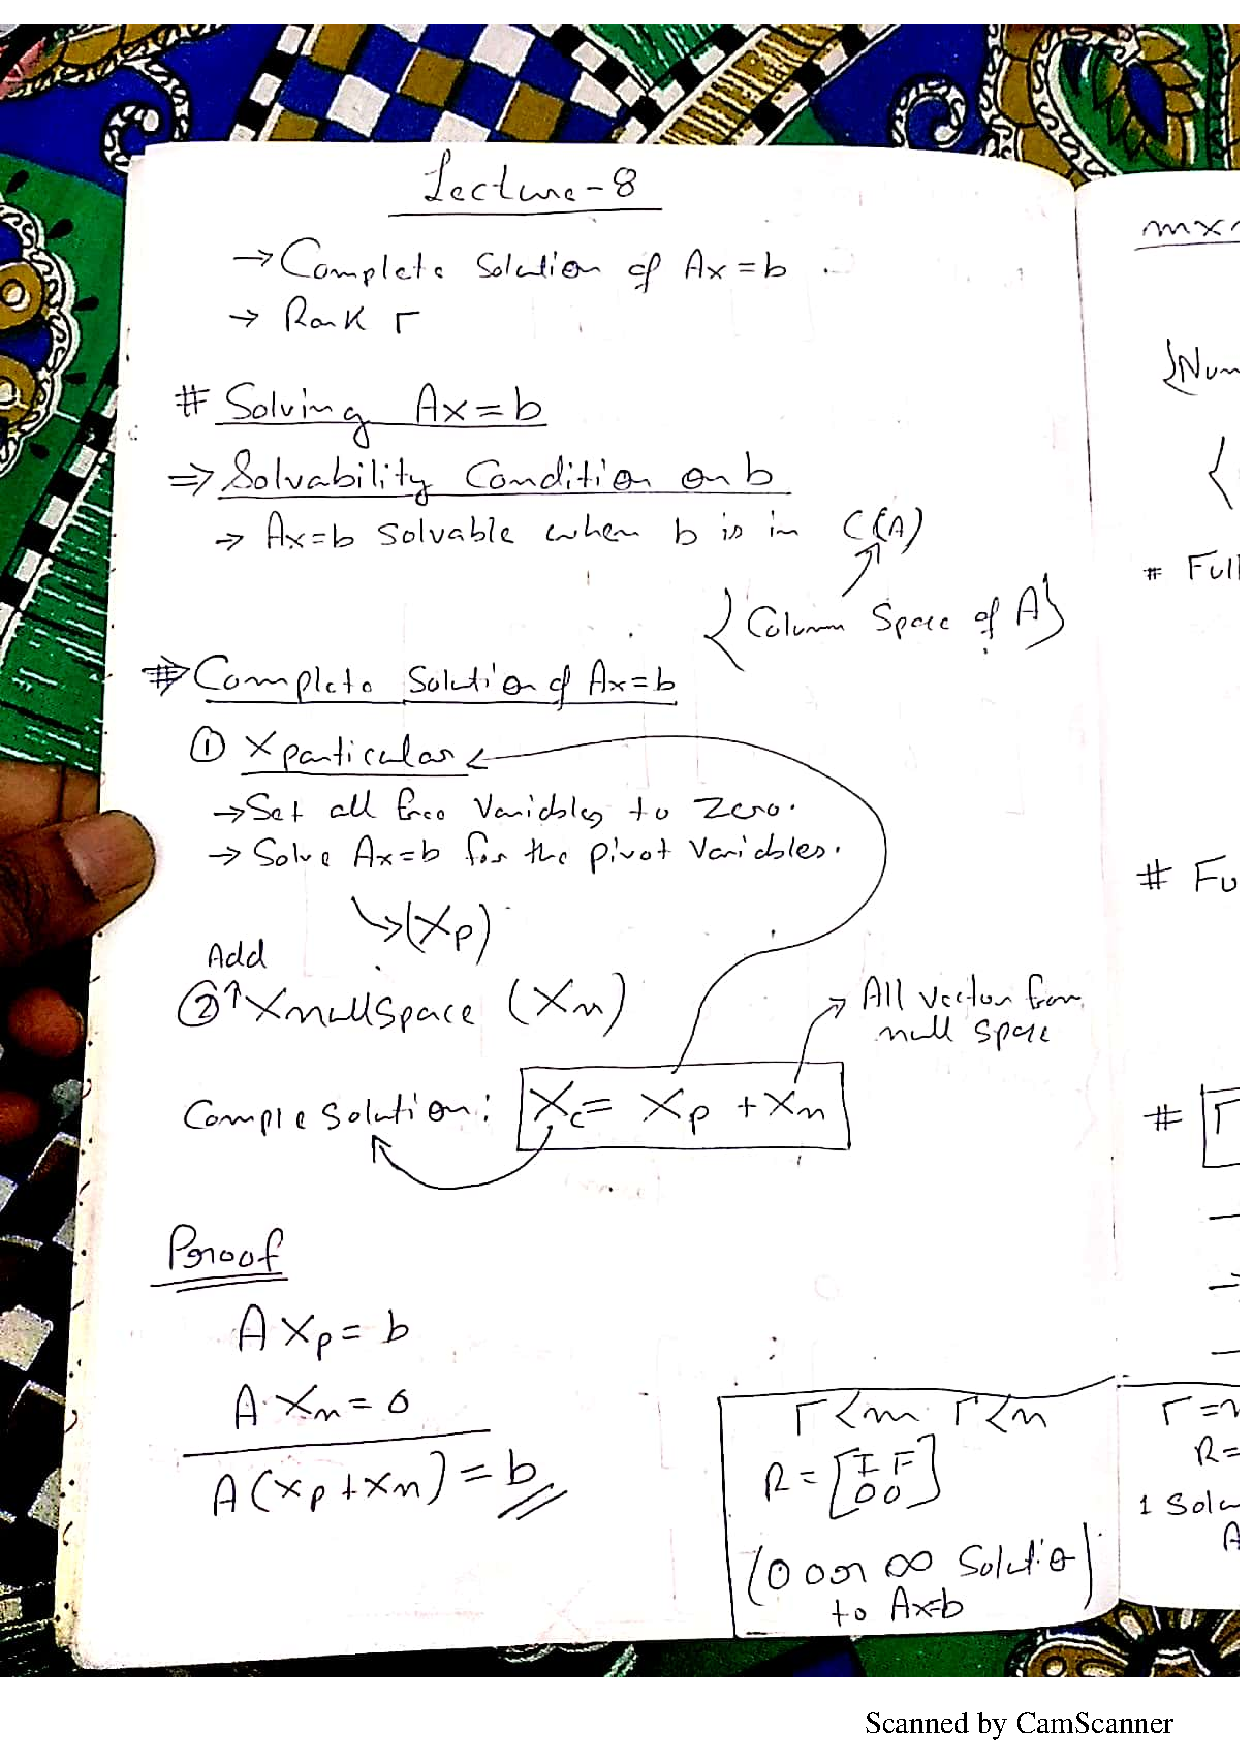
\includepdf[page=-]{./raw_files/8.pdf}

\chapter{Lecture 9}
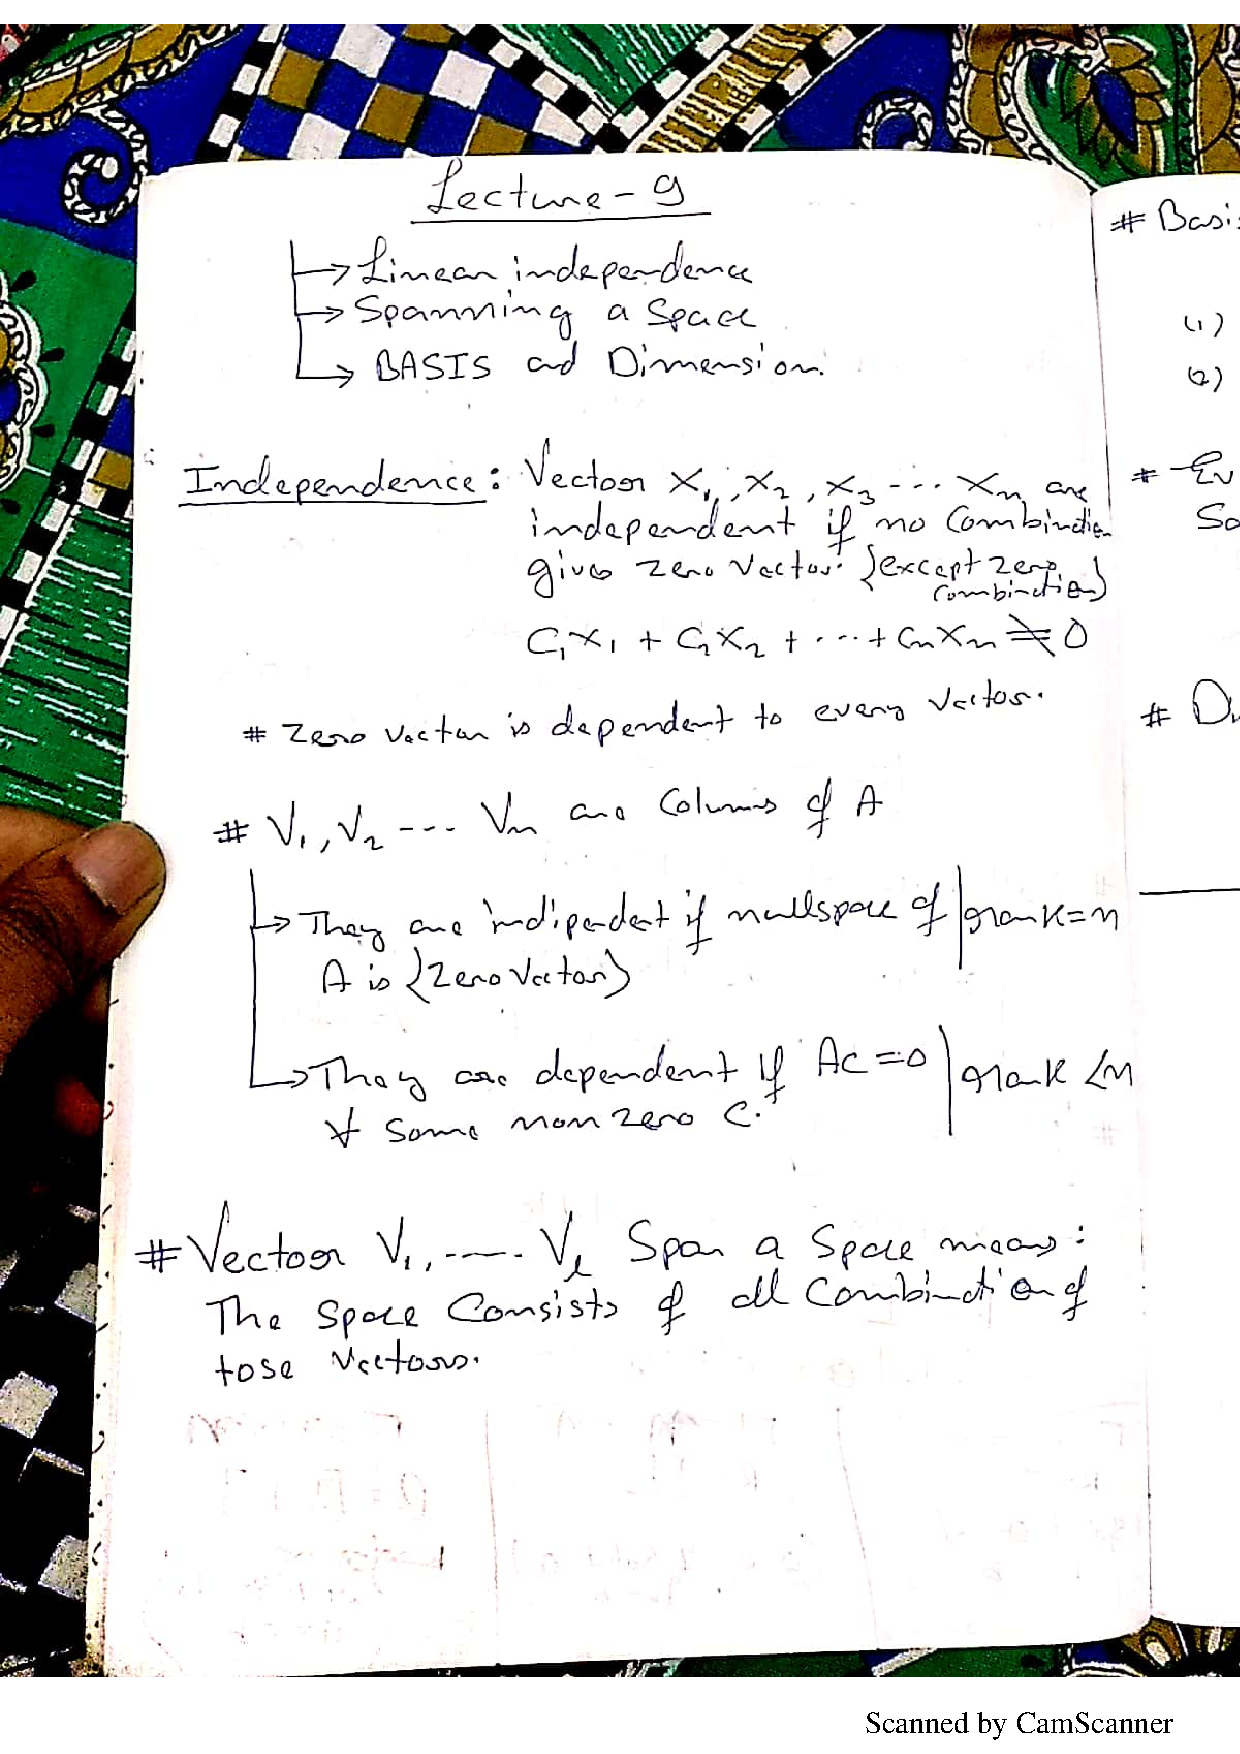
\includepdf[page=-]{./raw_files/9.pdf}

\chapter{Lecture 10}
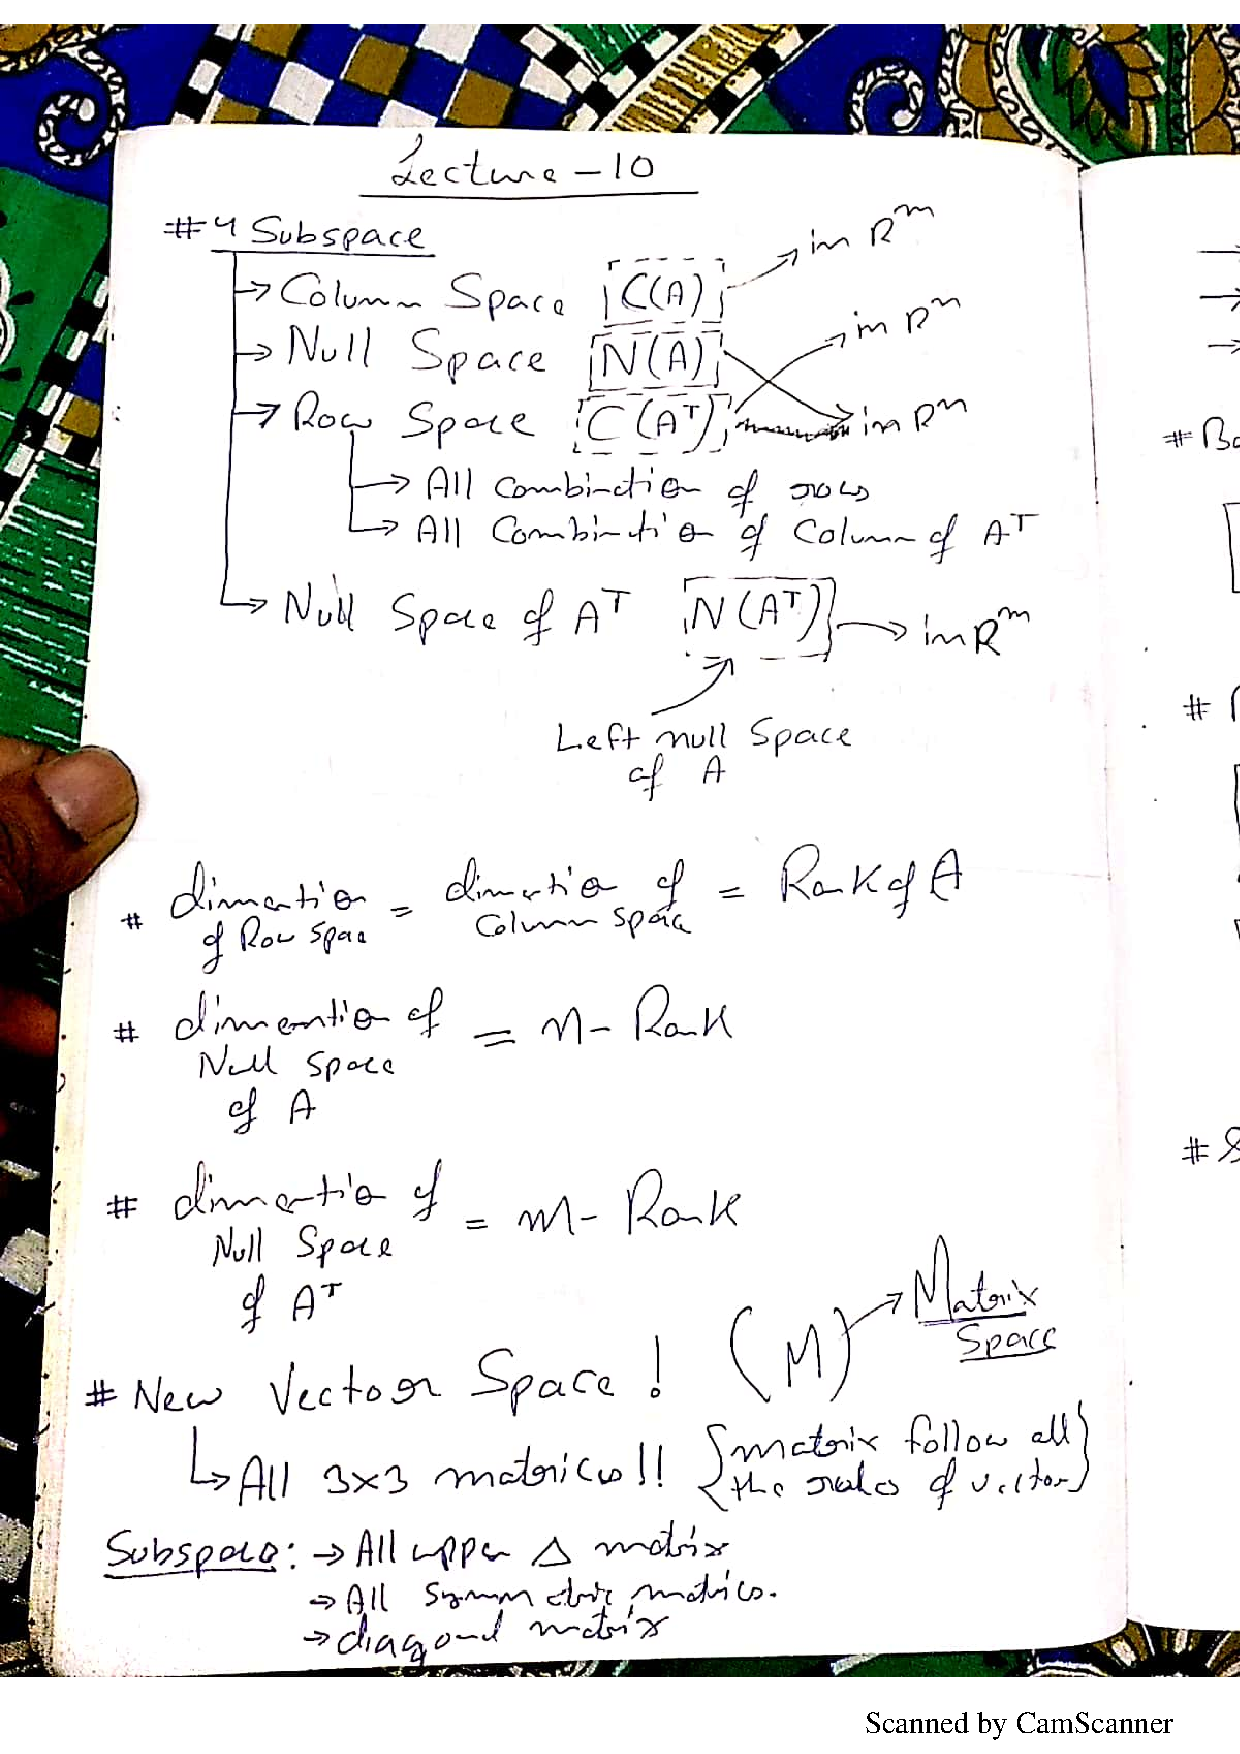
\includepdf[page=-]{./raw_files/10.pdf}

\chapter{Lecture 11}
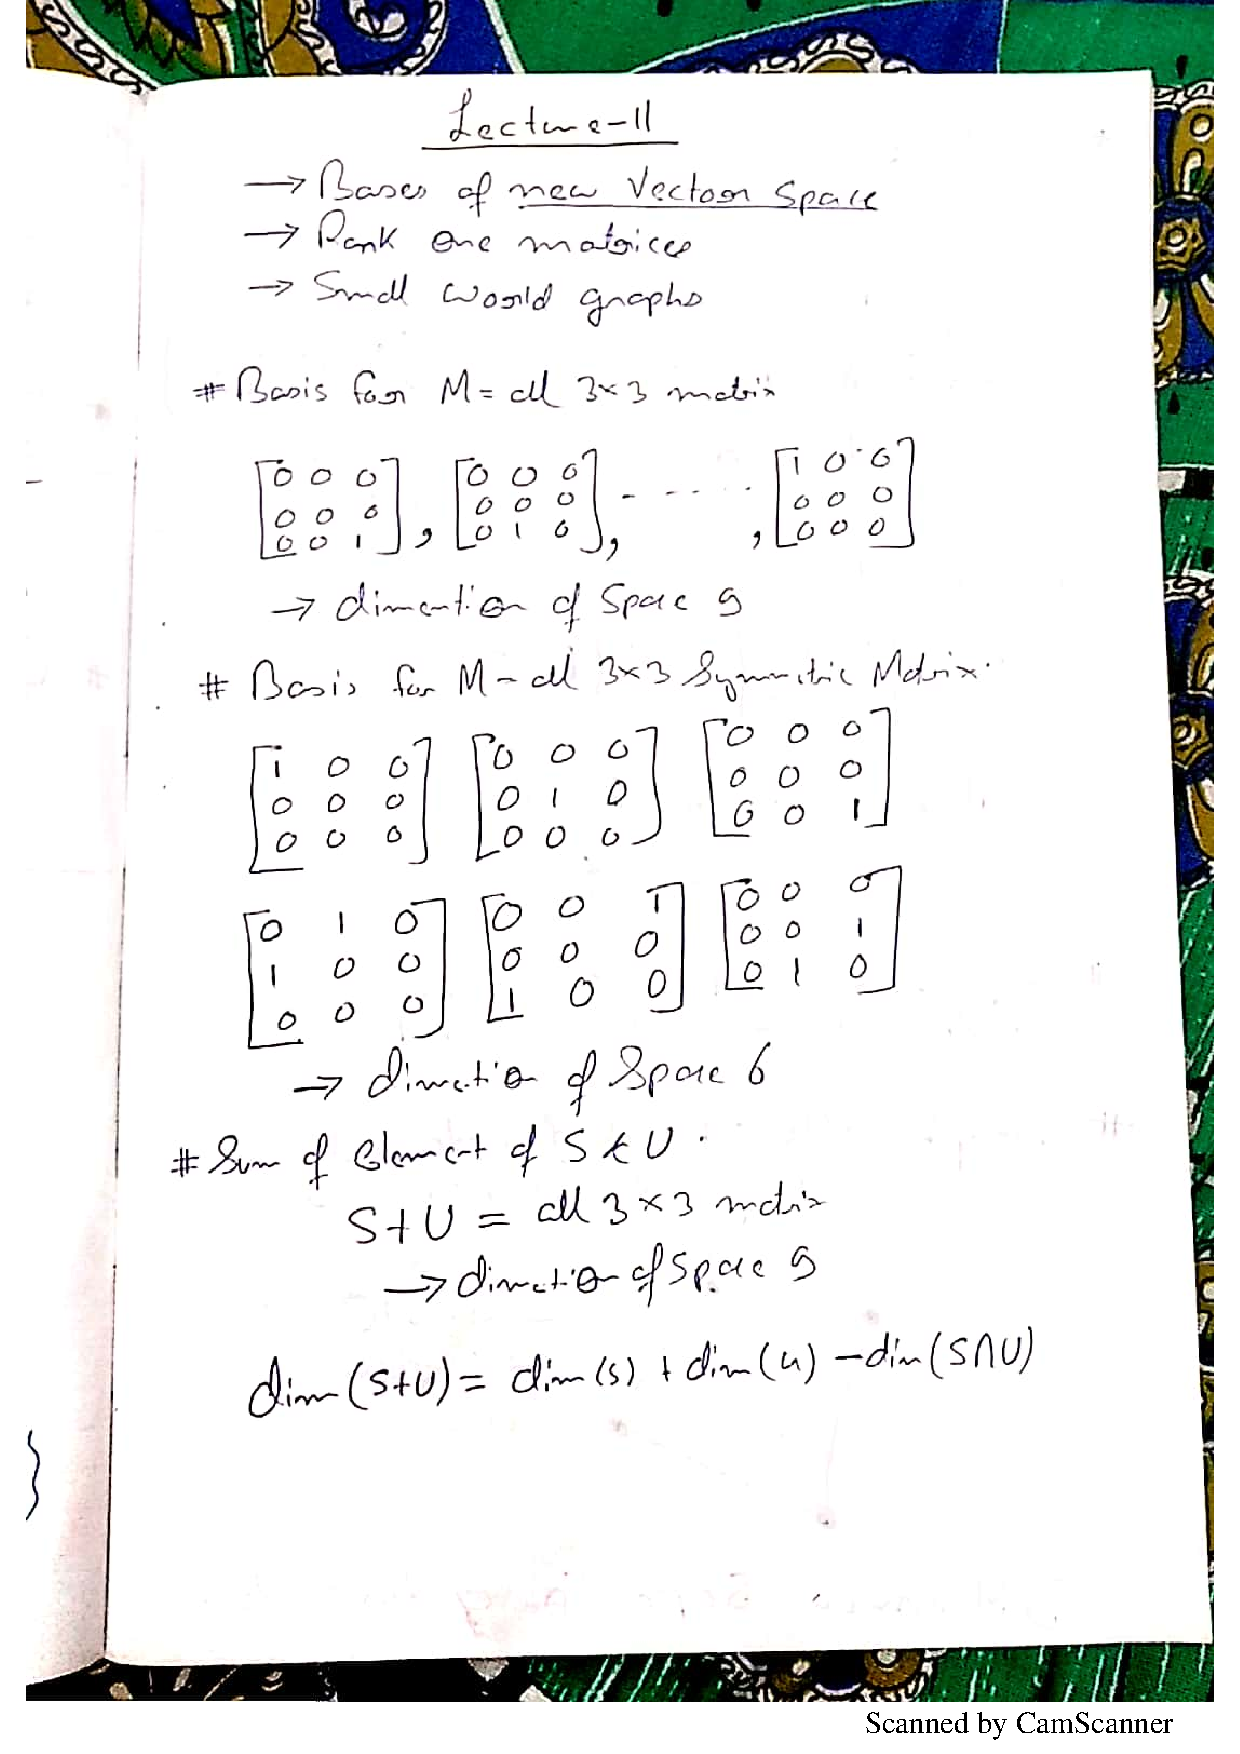
\includepdf[page=-]{./raw_files/11.pdf}

\chapter{Lecture 12}
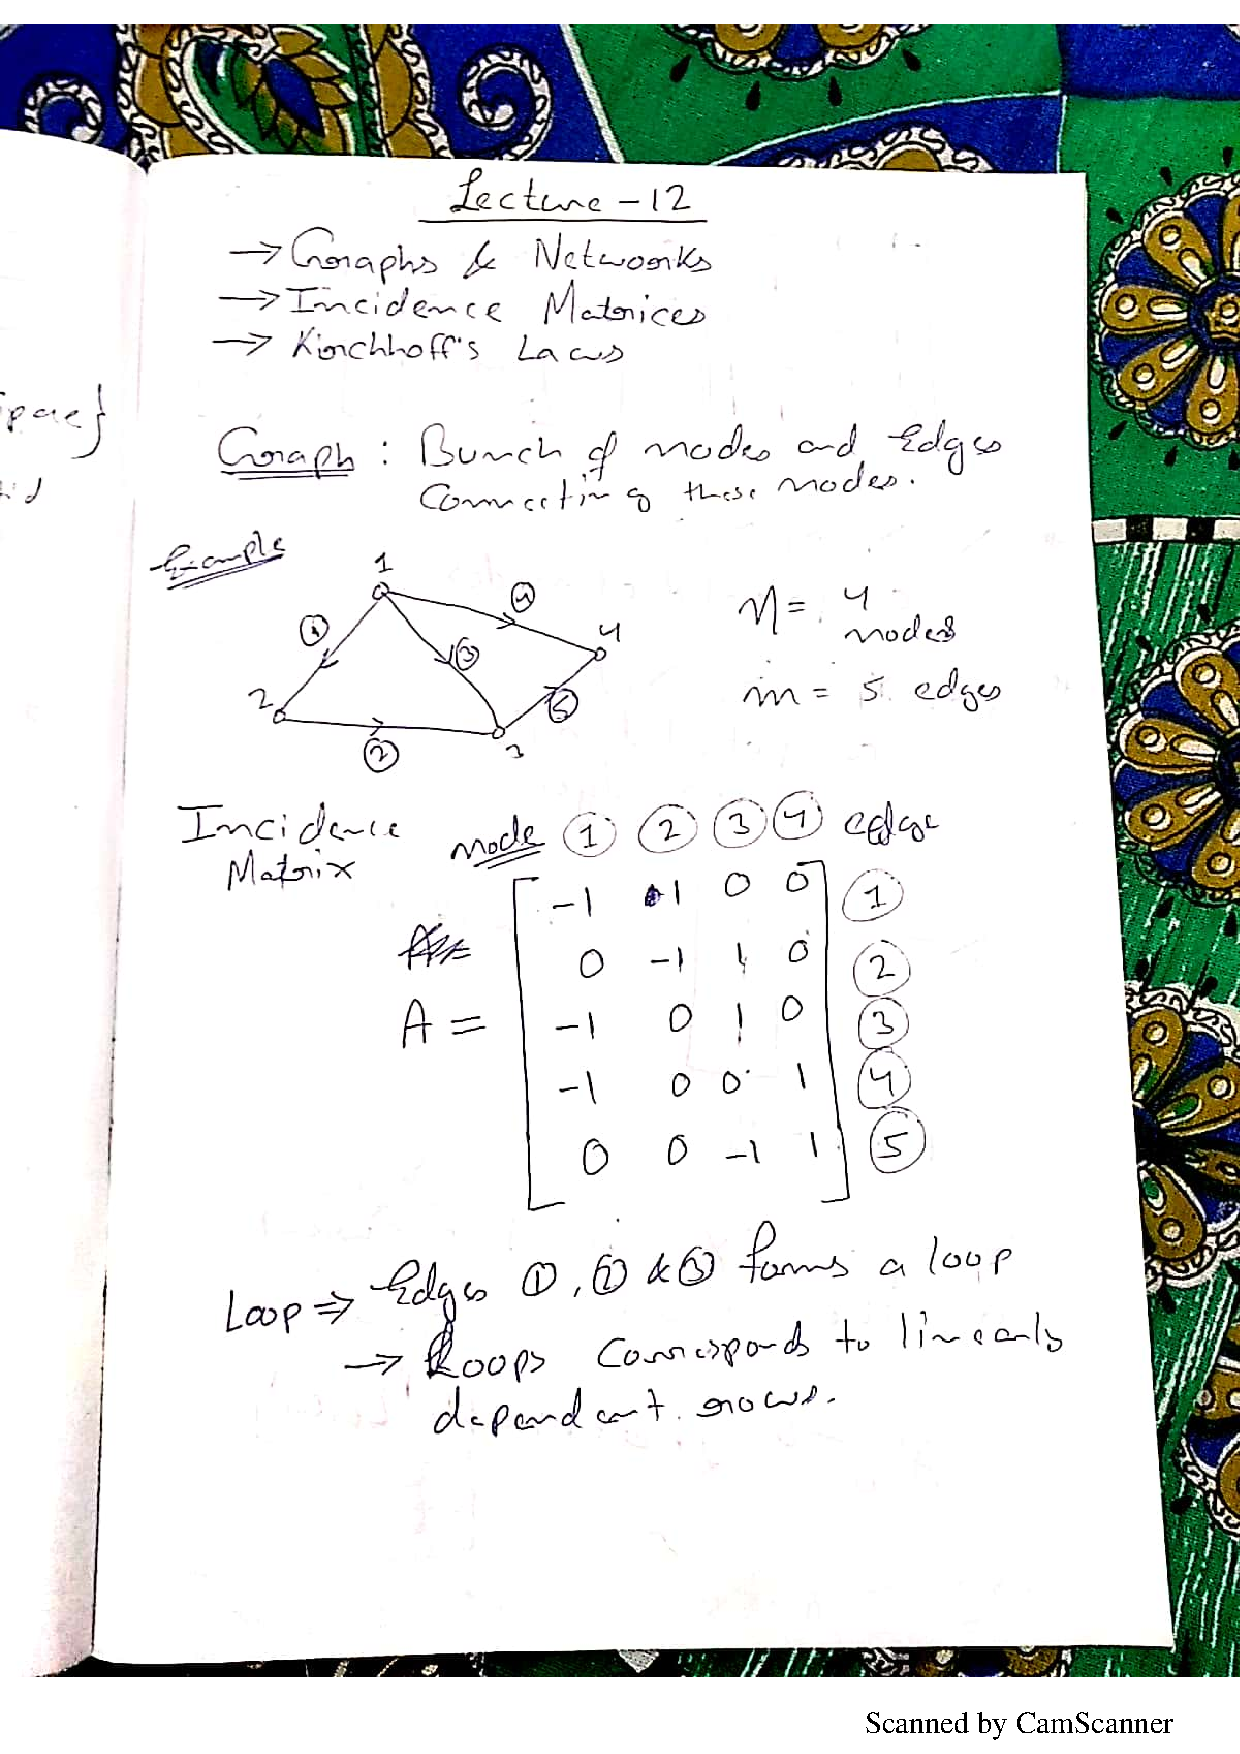
\includepdf[page=-]{./raw_files/12.pdf}

\chapter{Lecture 13}
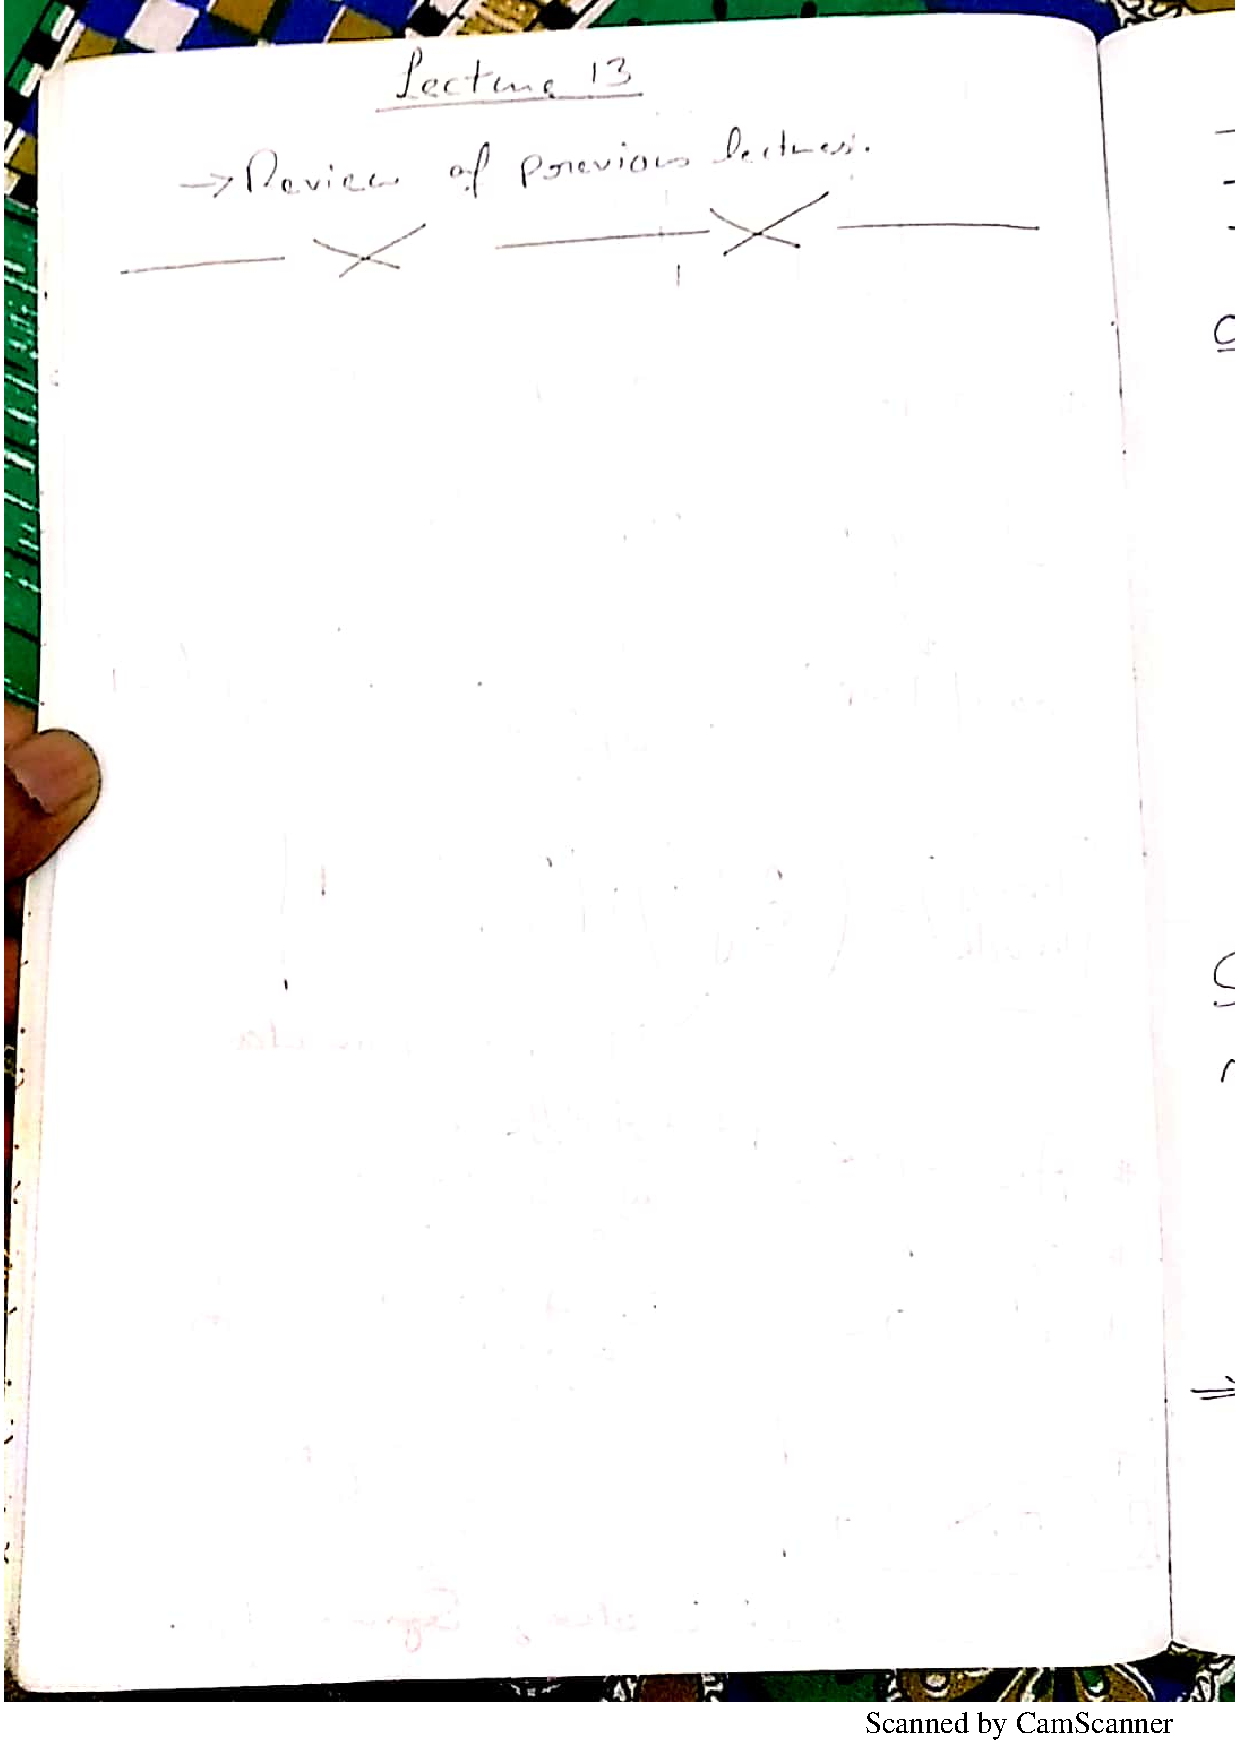
\includepdf[page=-]{./raw_files/13.pdf}

\chapter{Lecture 14}
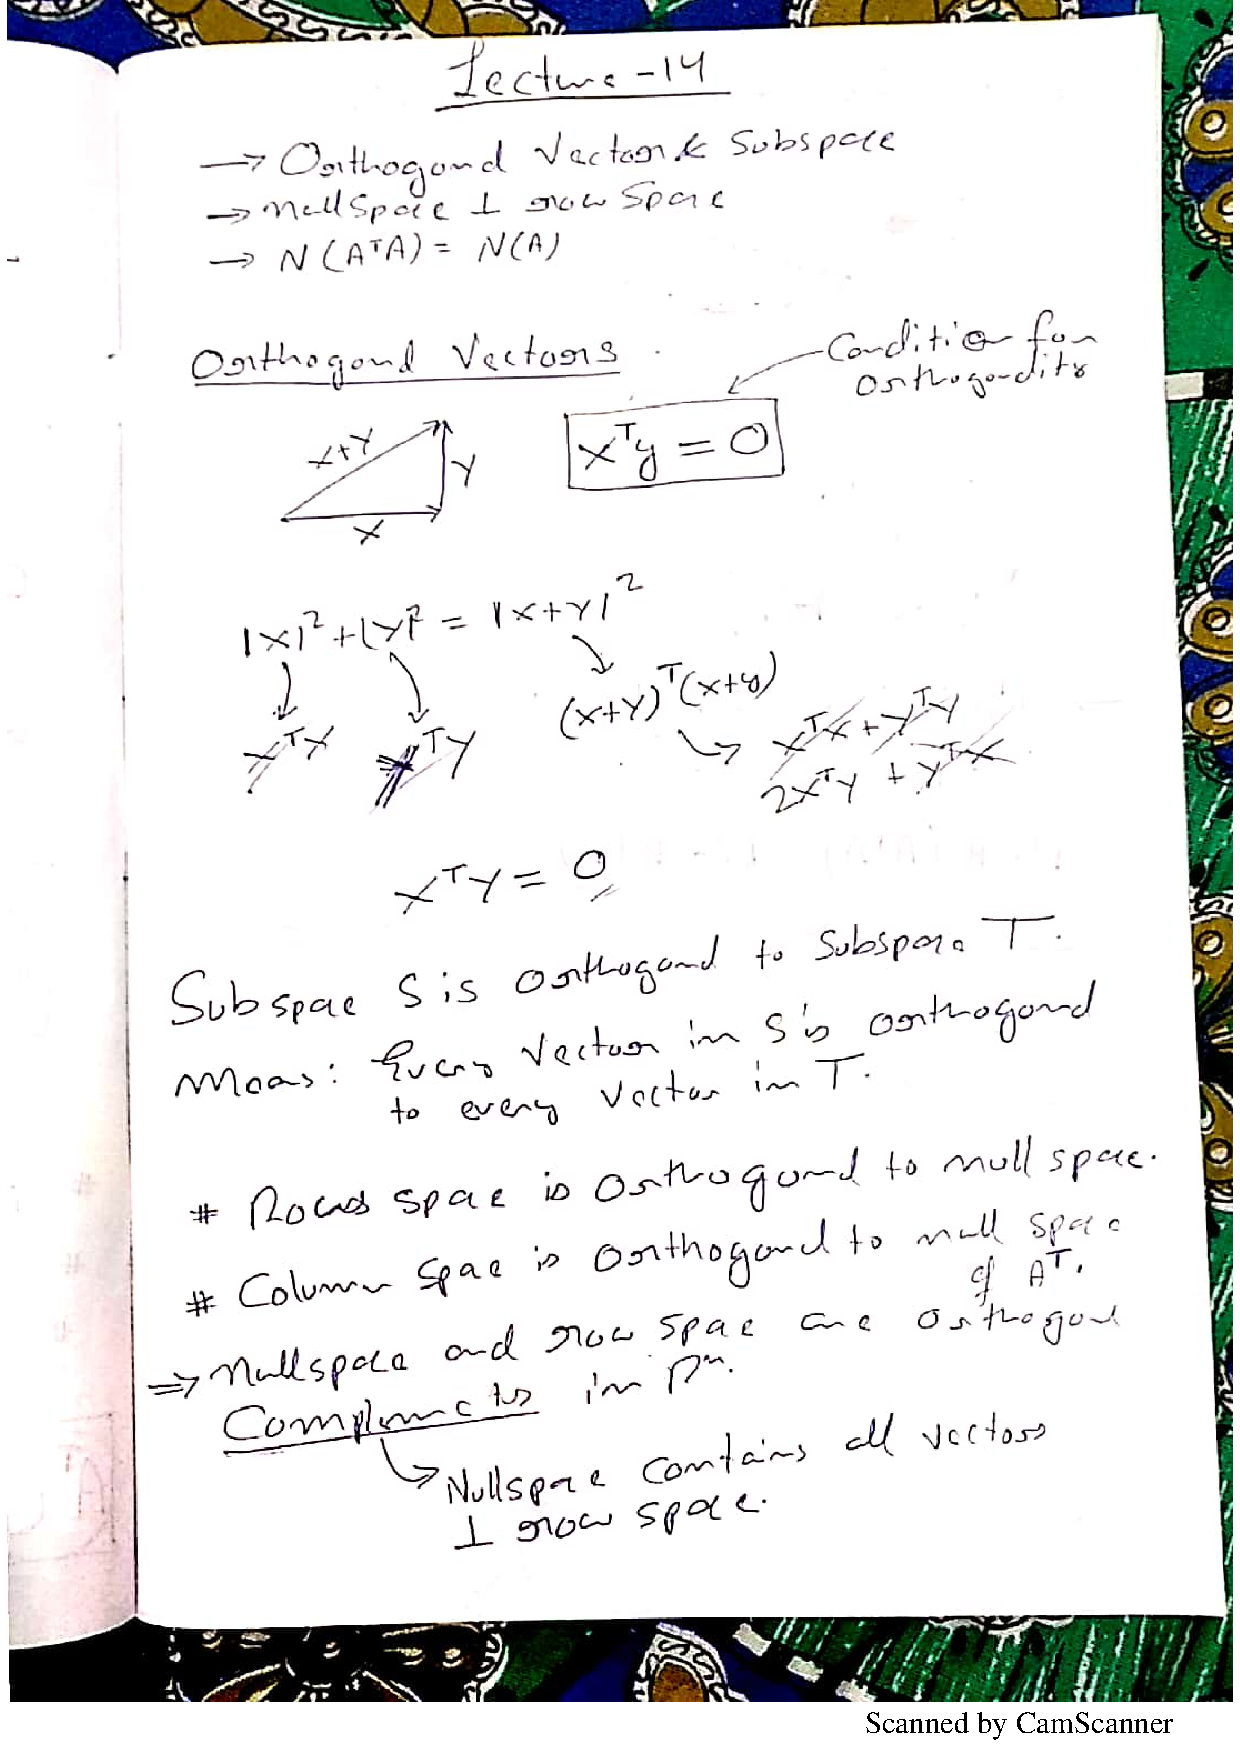
\includepdf[page=-]{./raw_files/14.pdf}

\chapter{Lecture 15}
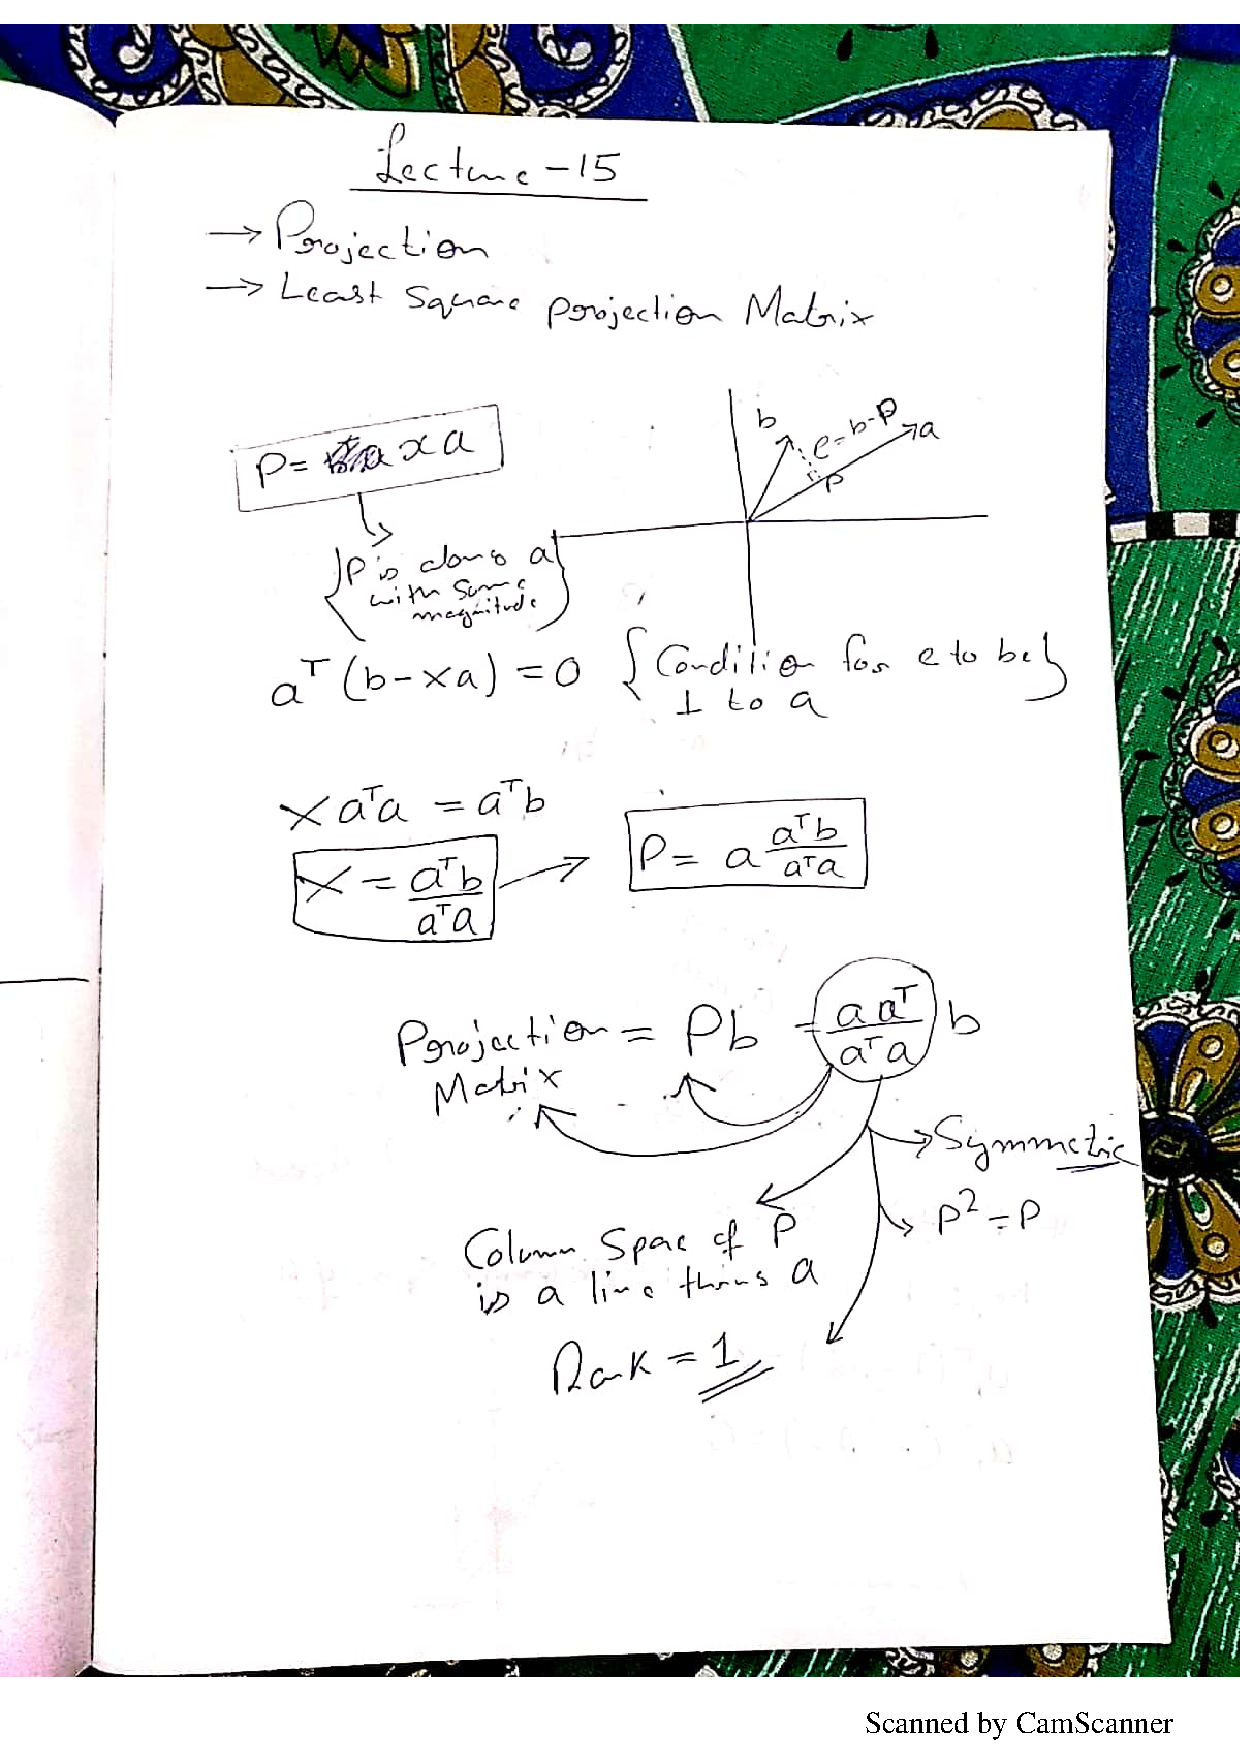
\includepdf[page=-]{./raw_files/15.pdf}

\chapter{Lecture 16}
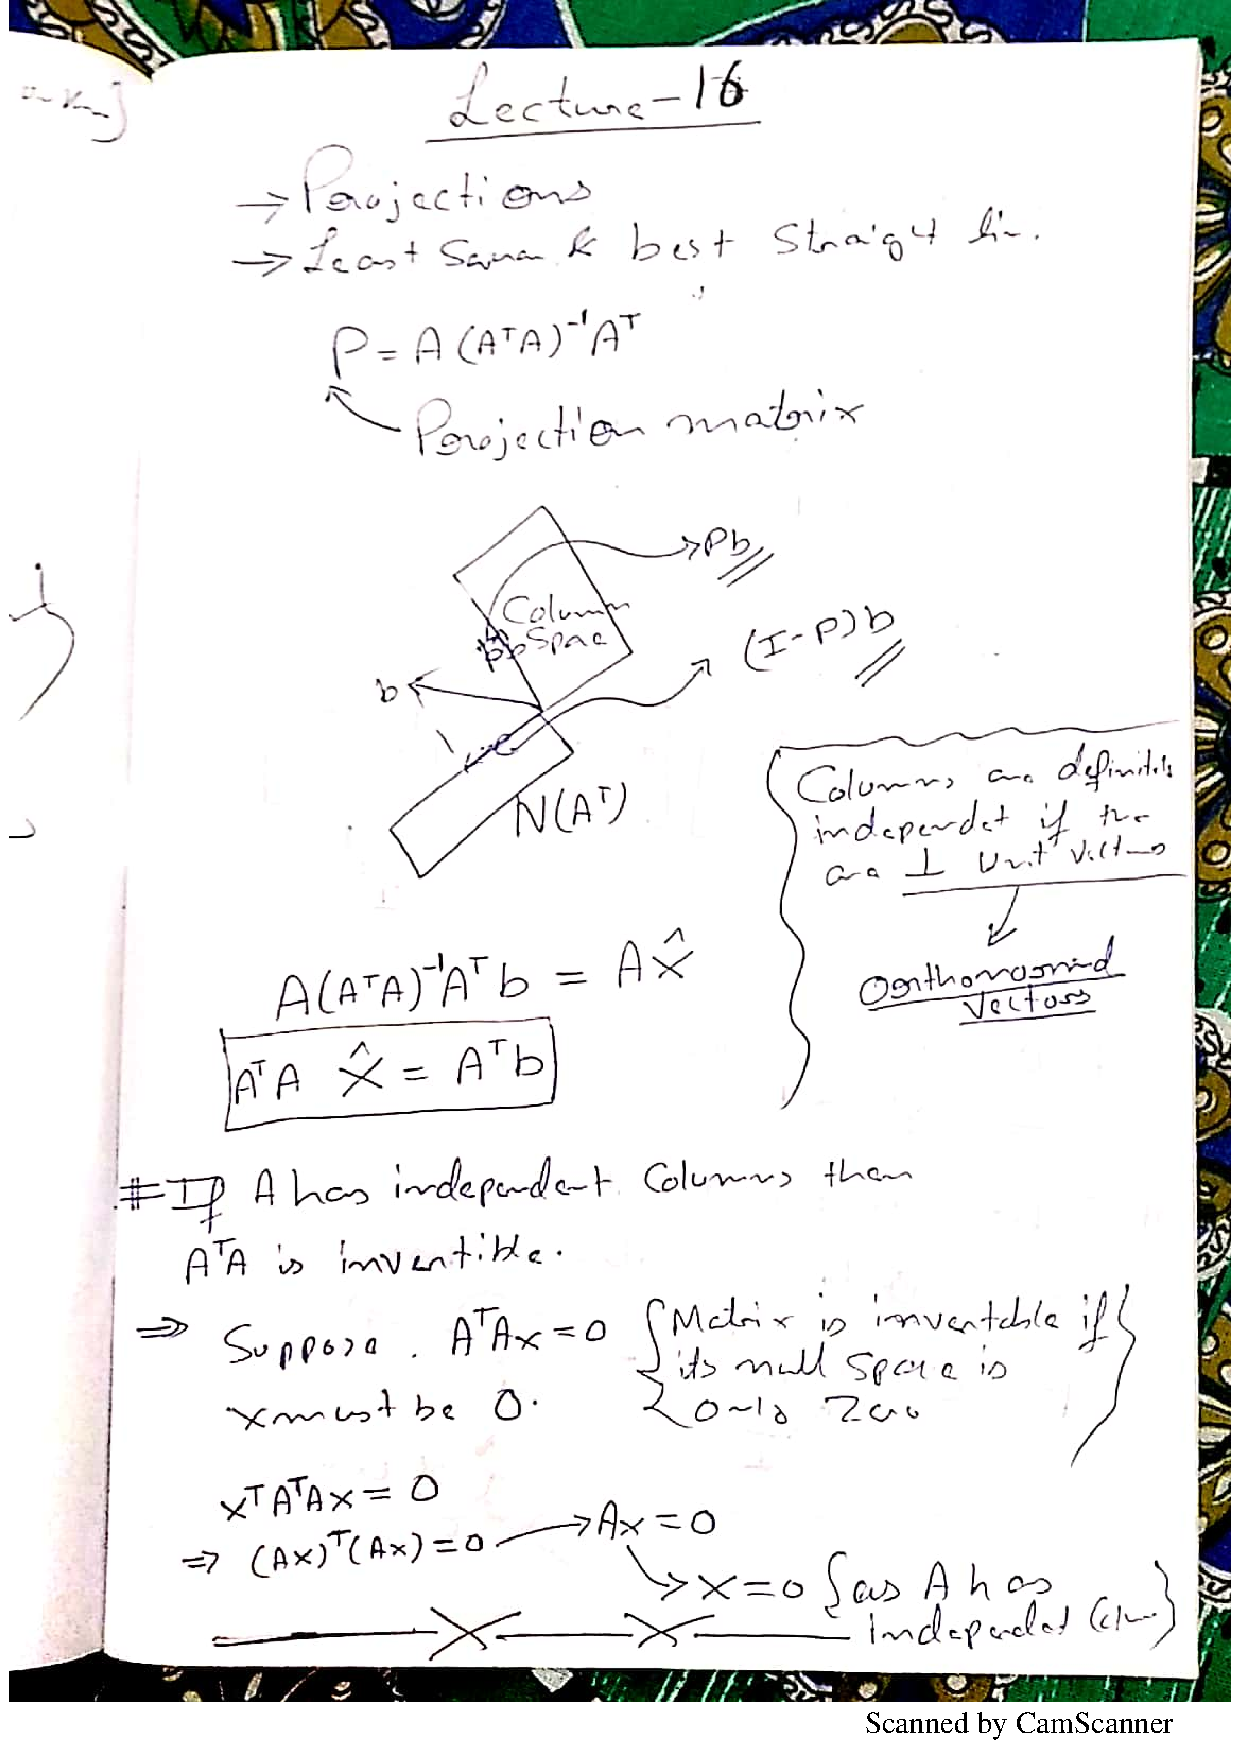
\includepdf[page=-]{./raw_files/16.pdf}

\chapter{Lecture 17}
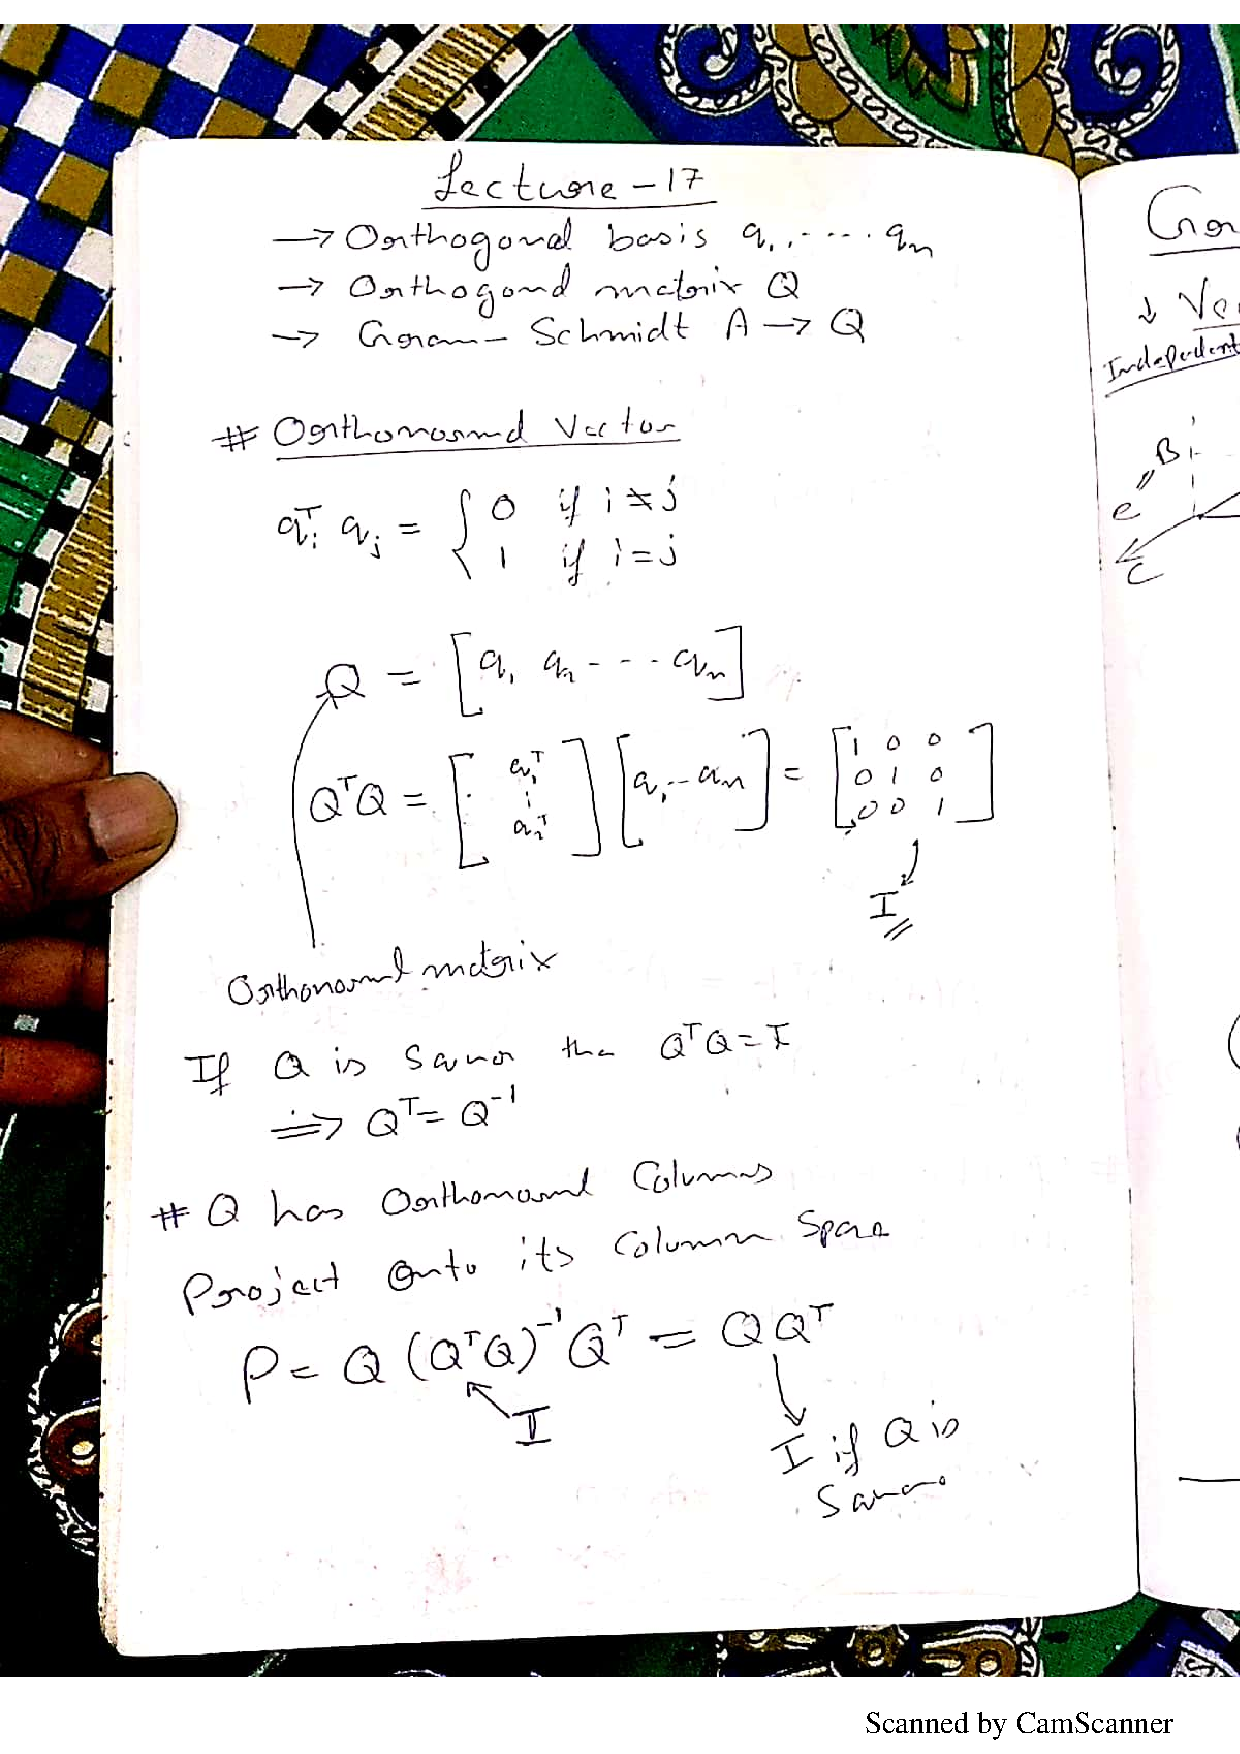
\includepdf[page=-]{./raw_files/17.pdf}

\chapter{Lecture 18}
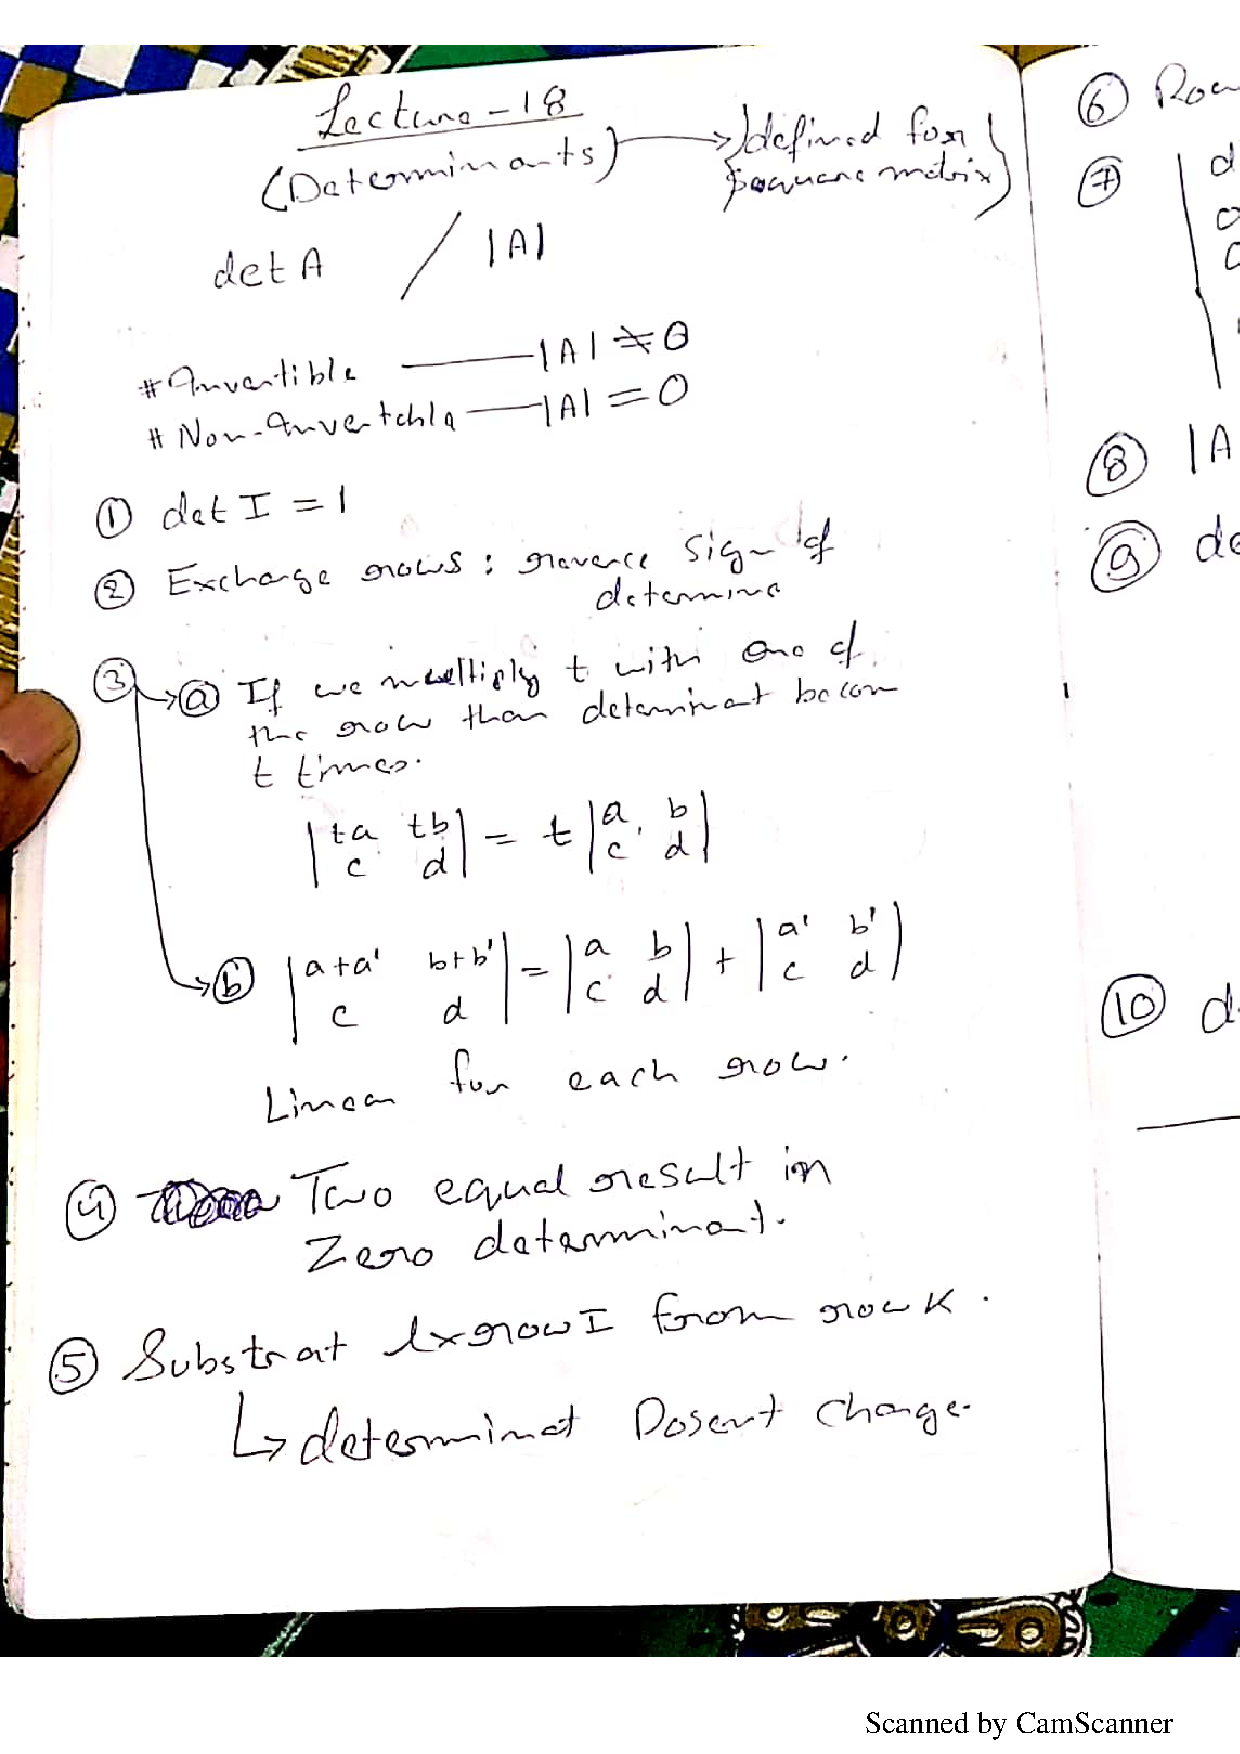
\includepdf[page=-]{./raw_files/18.pdf}

\chapter{Lecture 19}
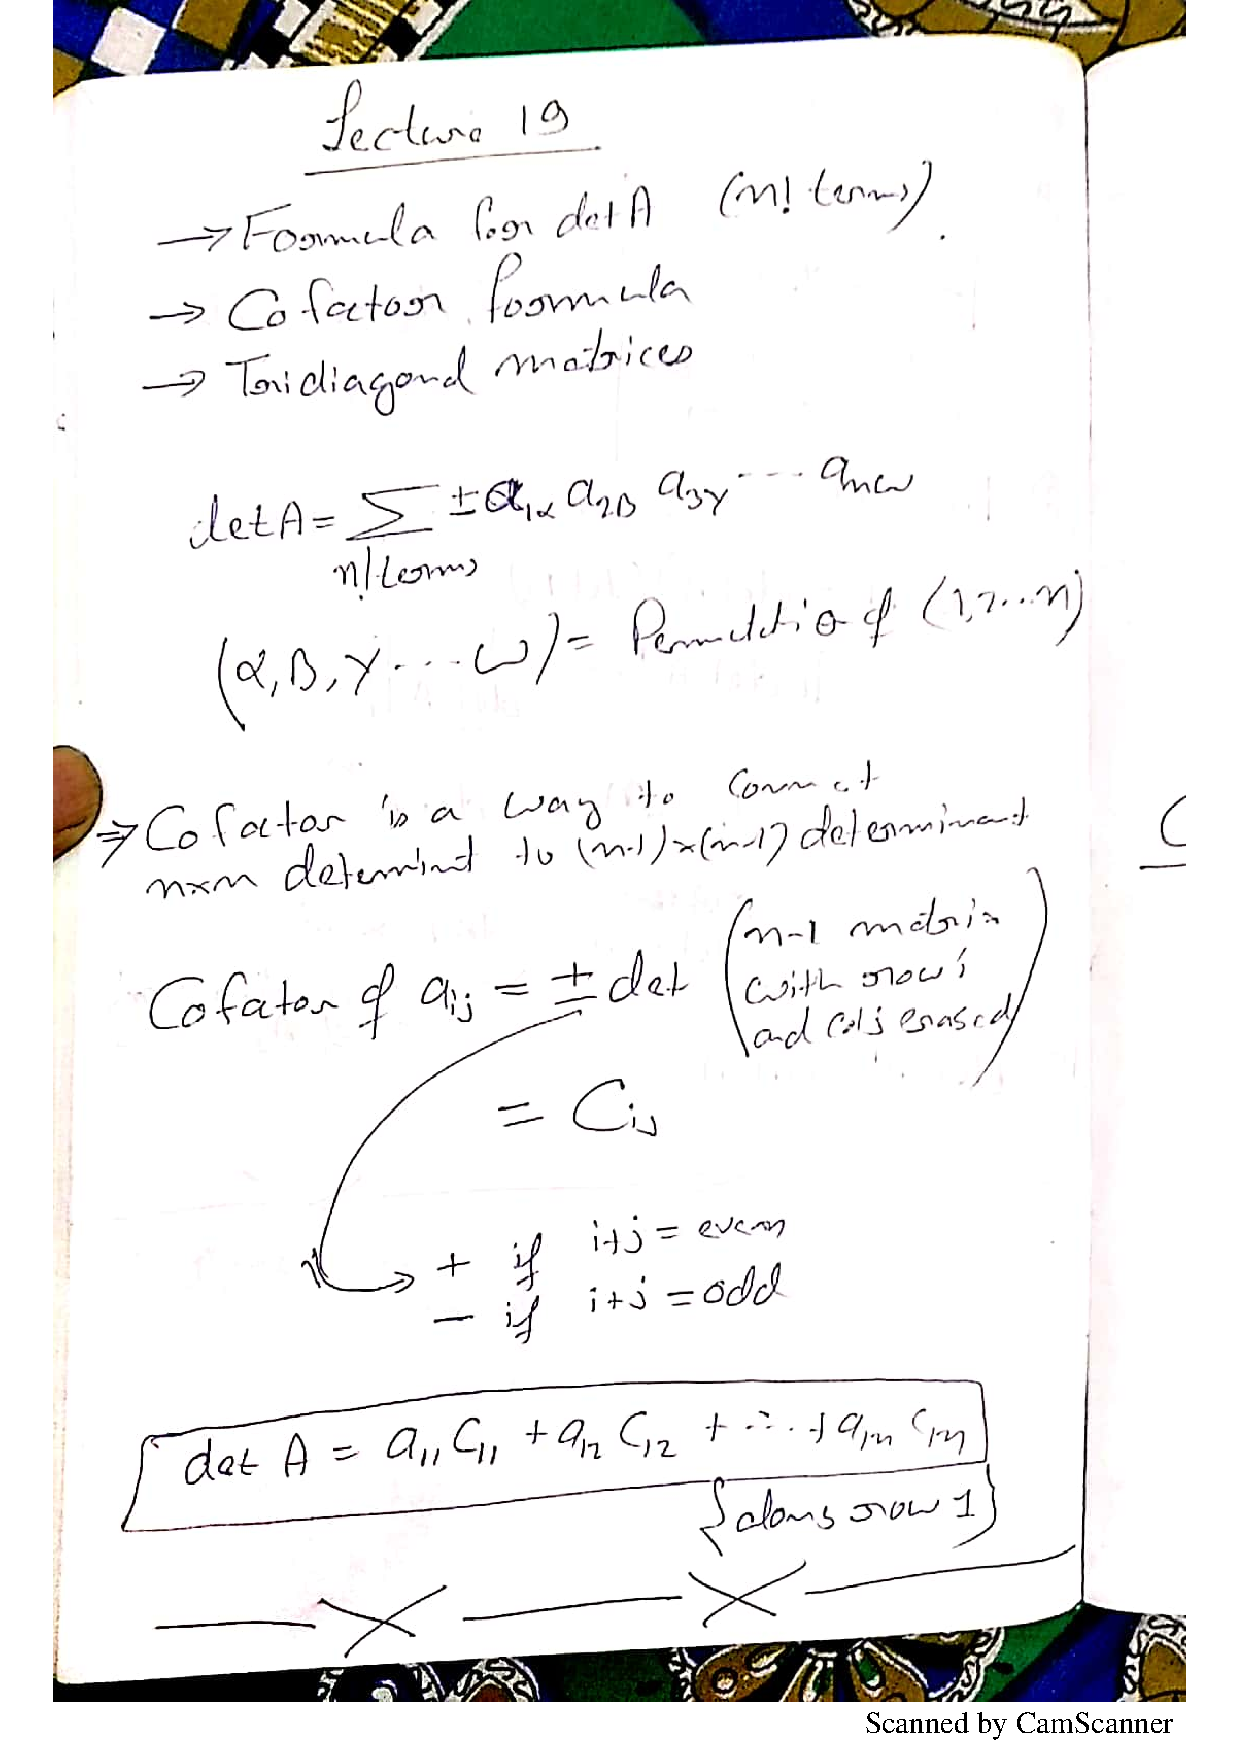
\includepdf[page=-]{./raw_files/19.pdf}

\chapter{Lecture 20}
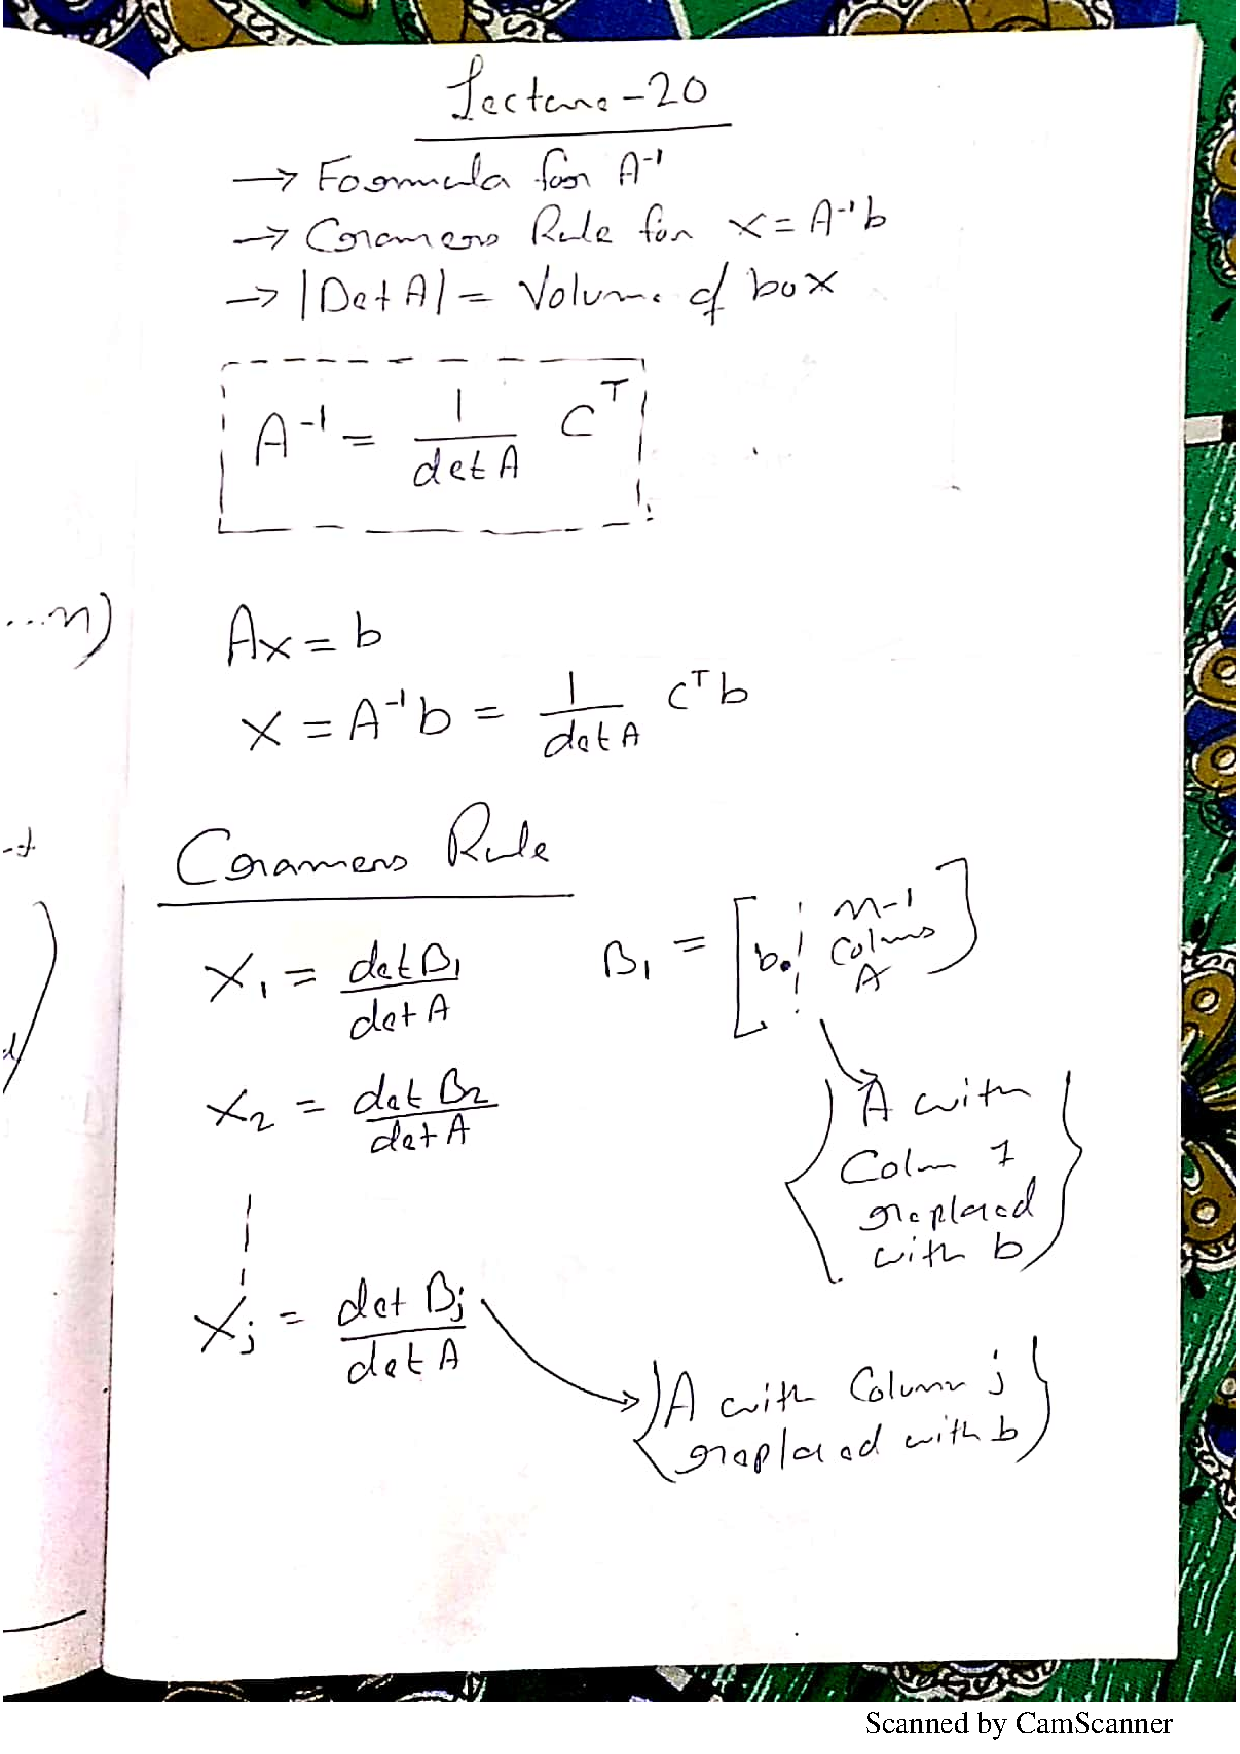
\includepdf[page=-]{./raw_files/20.pdf}

\chapter{Lecture 21}
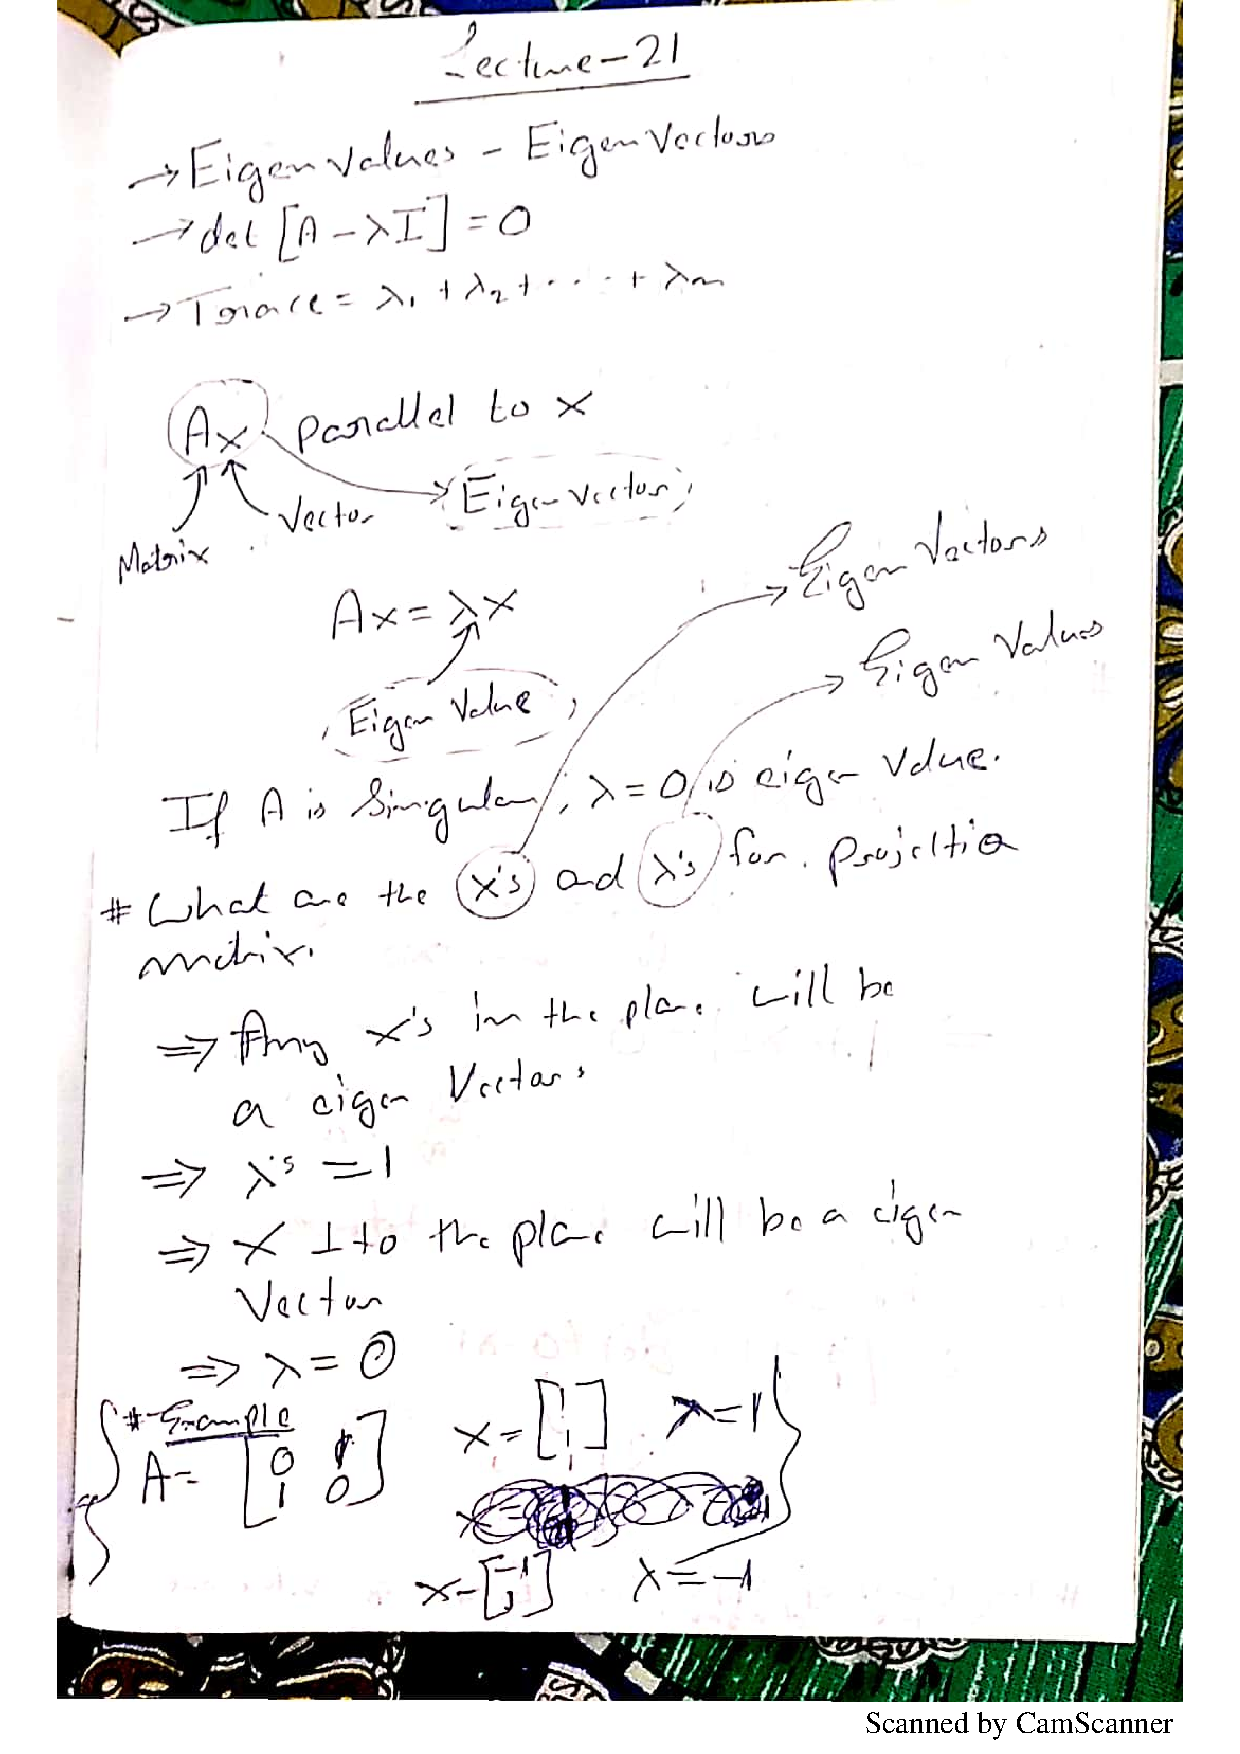
\includepdf[page=-]{./raw_files/21.pdf}

\chapter{Lecture 22}
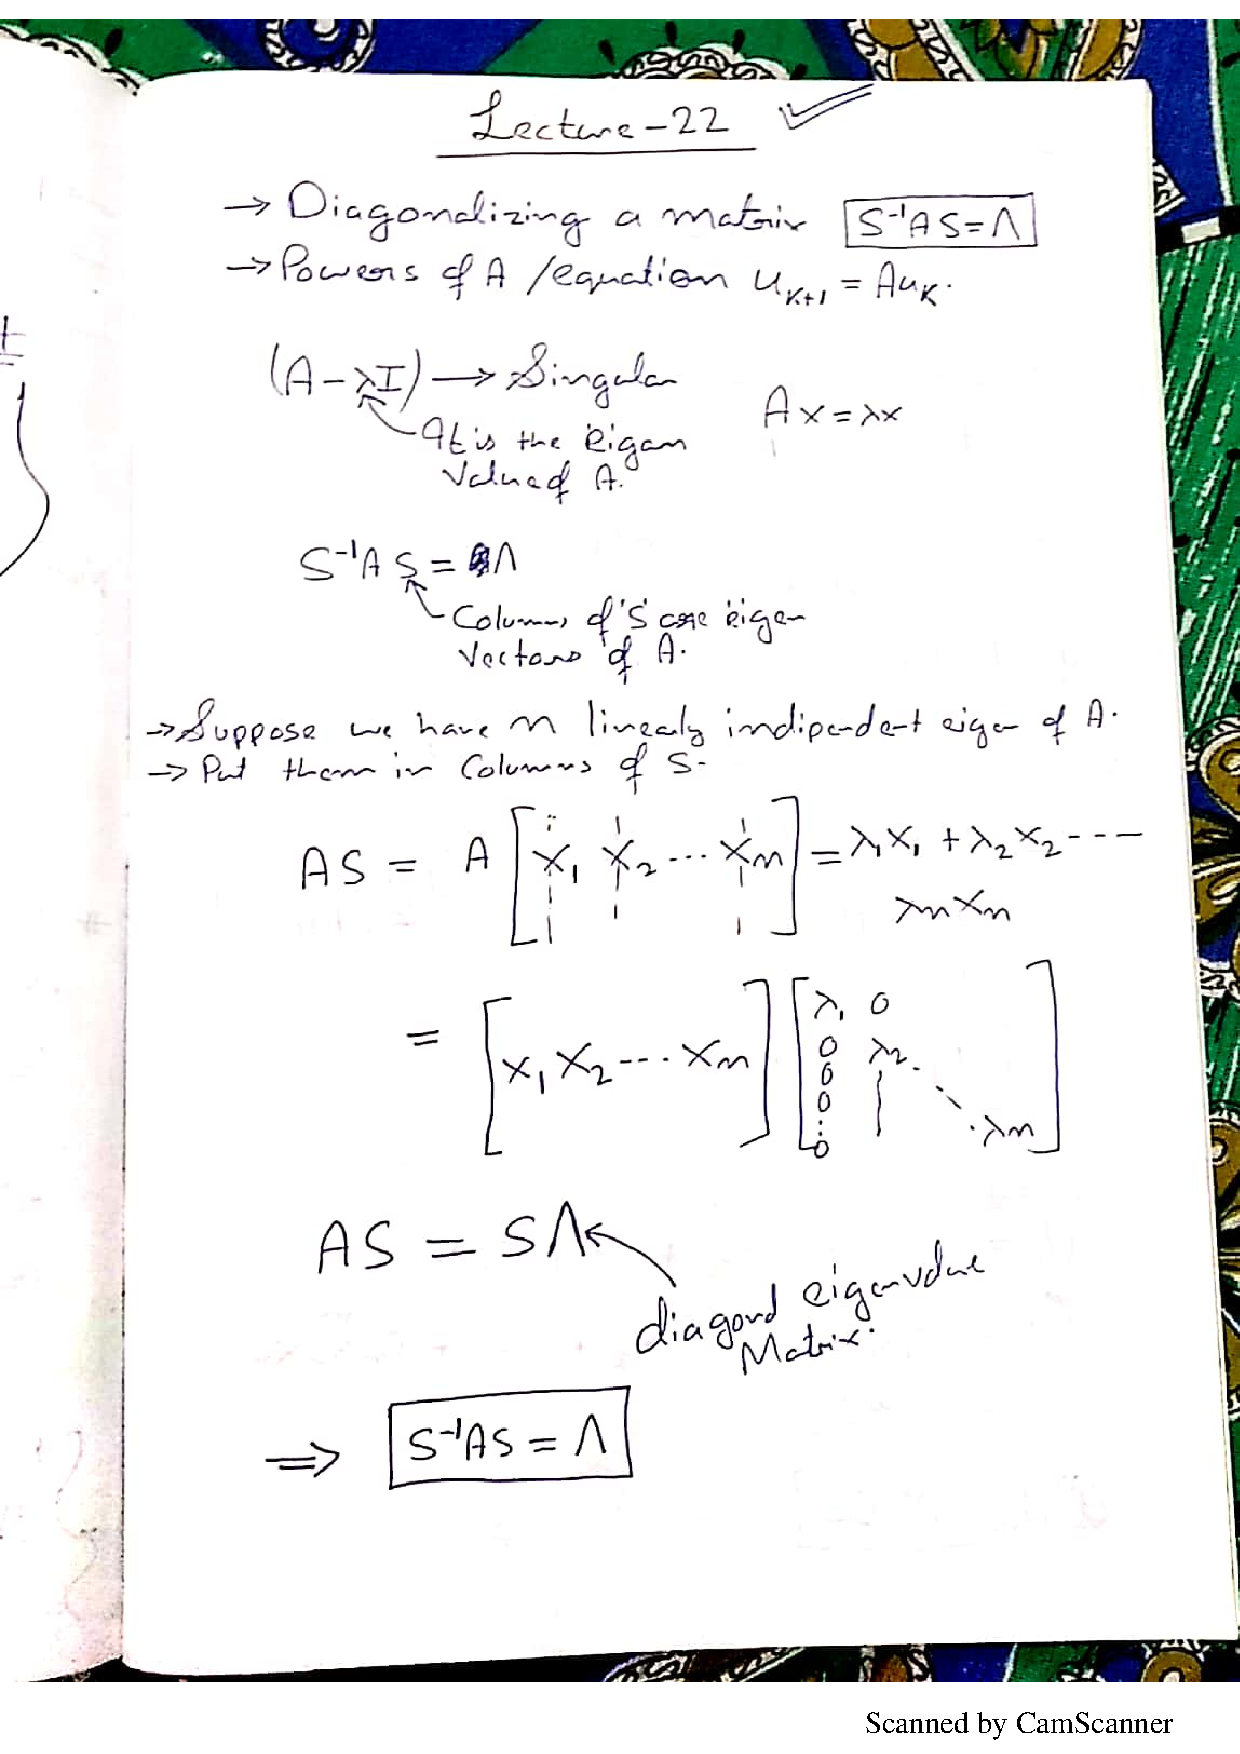
\includepdf[page=-]{./raw_files/22.pdf}

\chapter{Lecture 23}
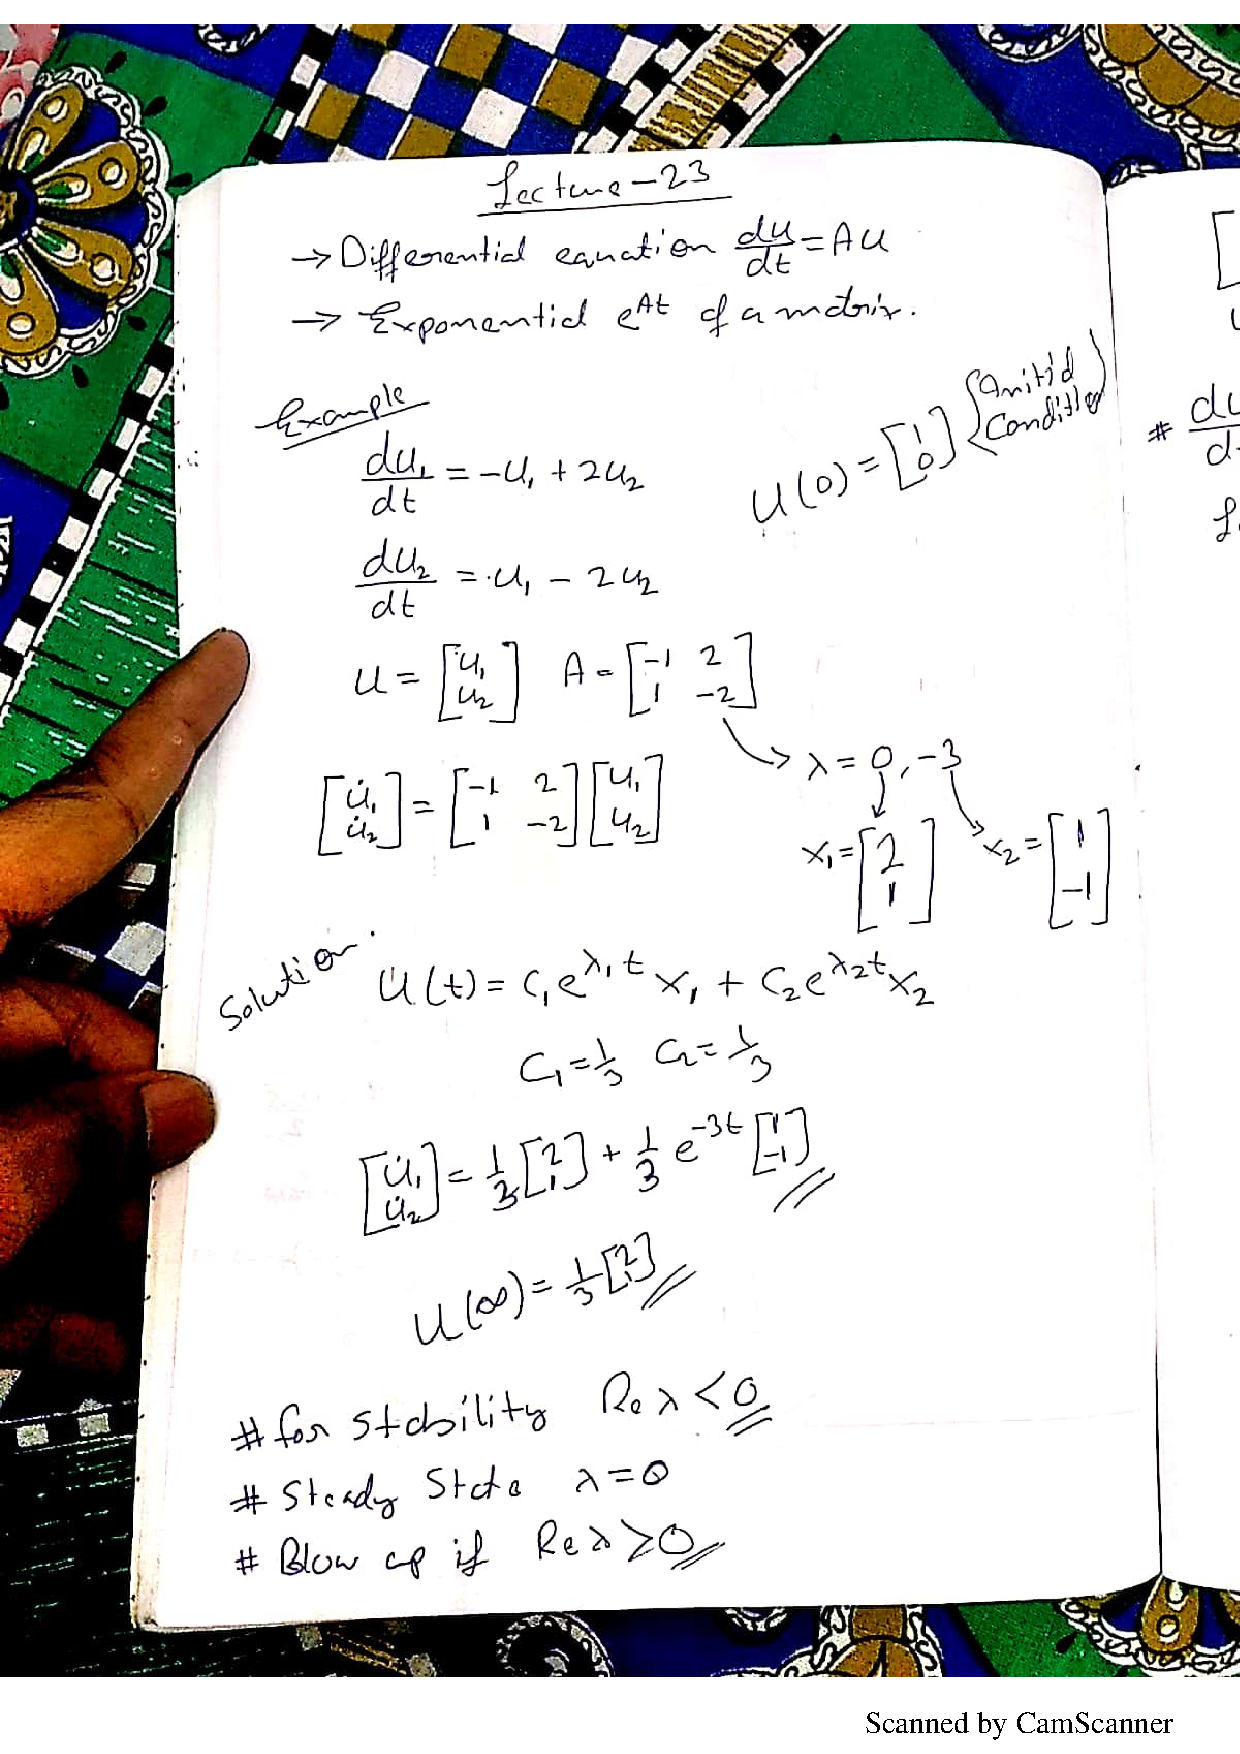
\includepdf[page=-]{./raw_files/23.pdf}

\chapter{Lecture 24}
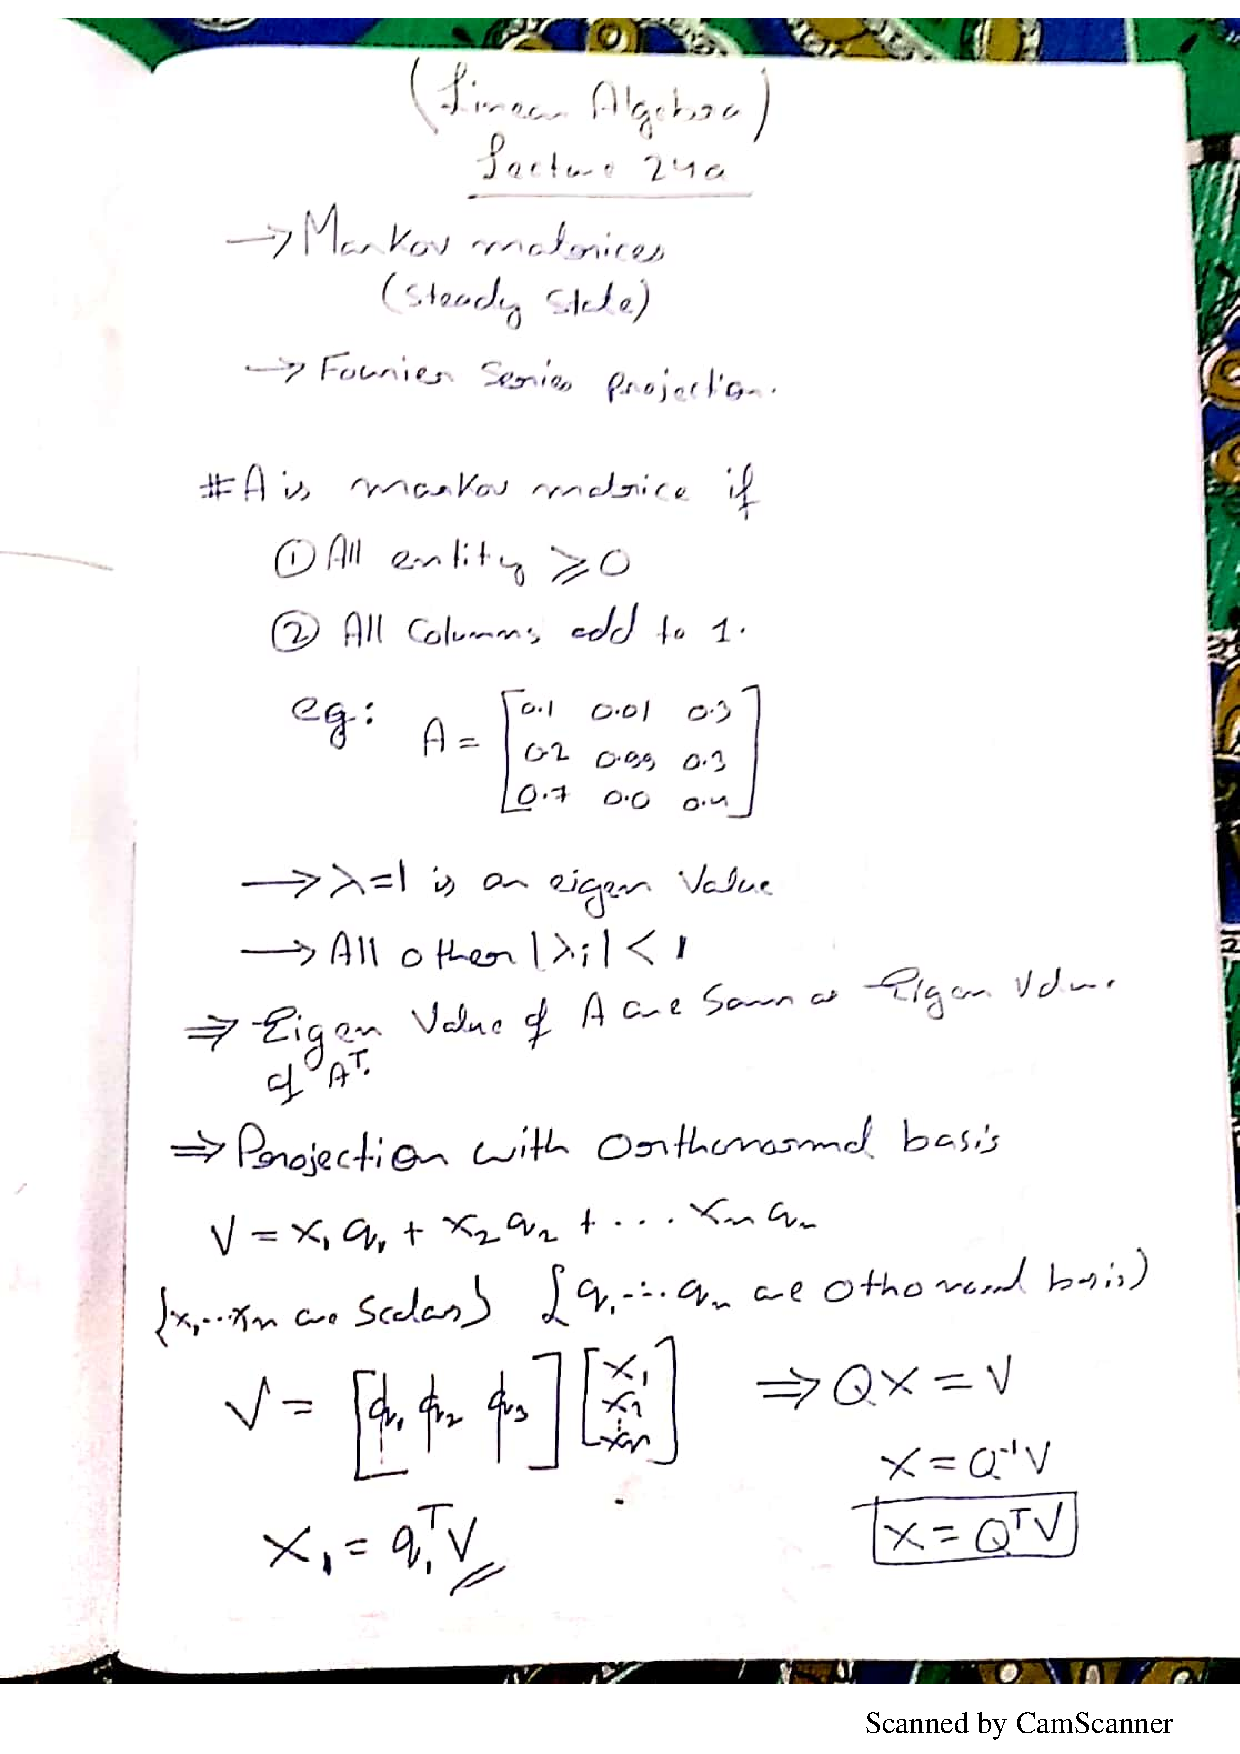
\includepdf[page=-]{./raw_files/24.pdf}

\chapter{Lecture 25}
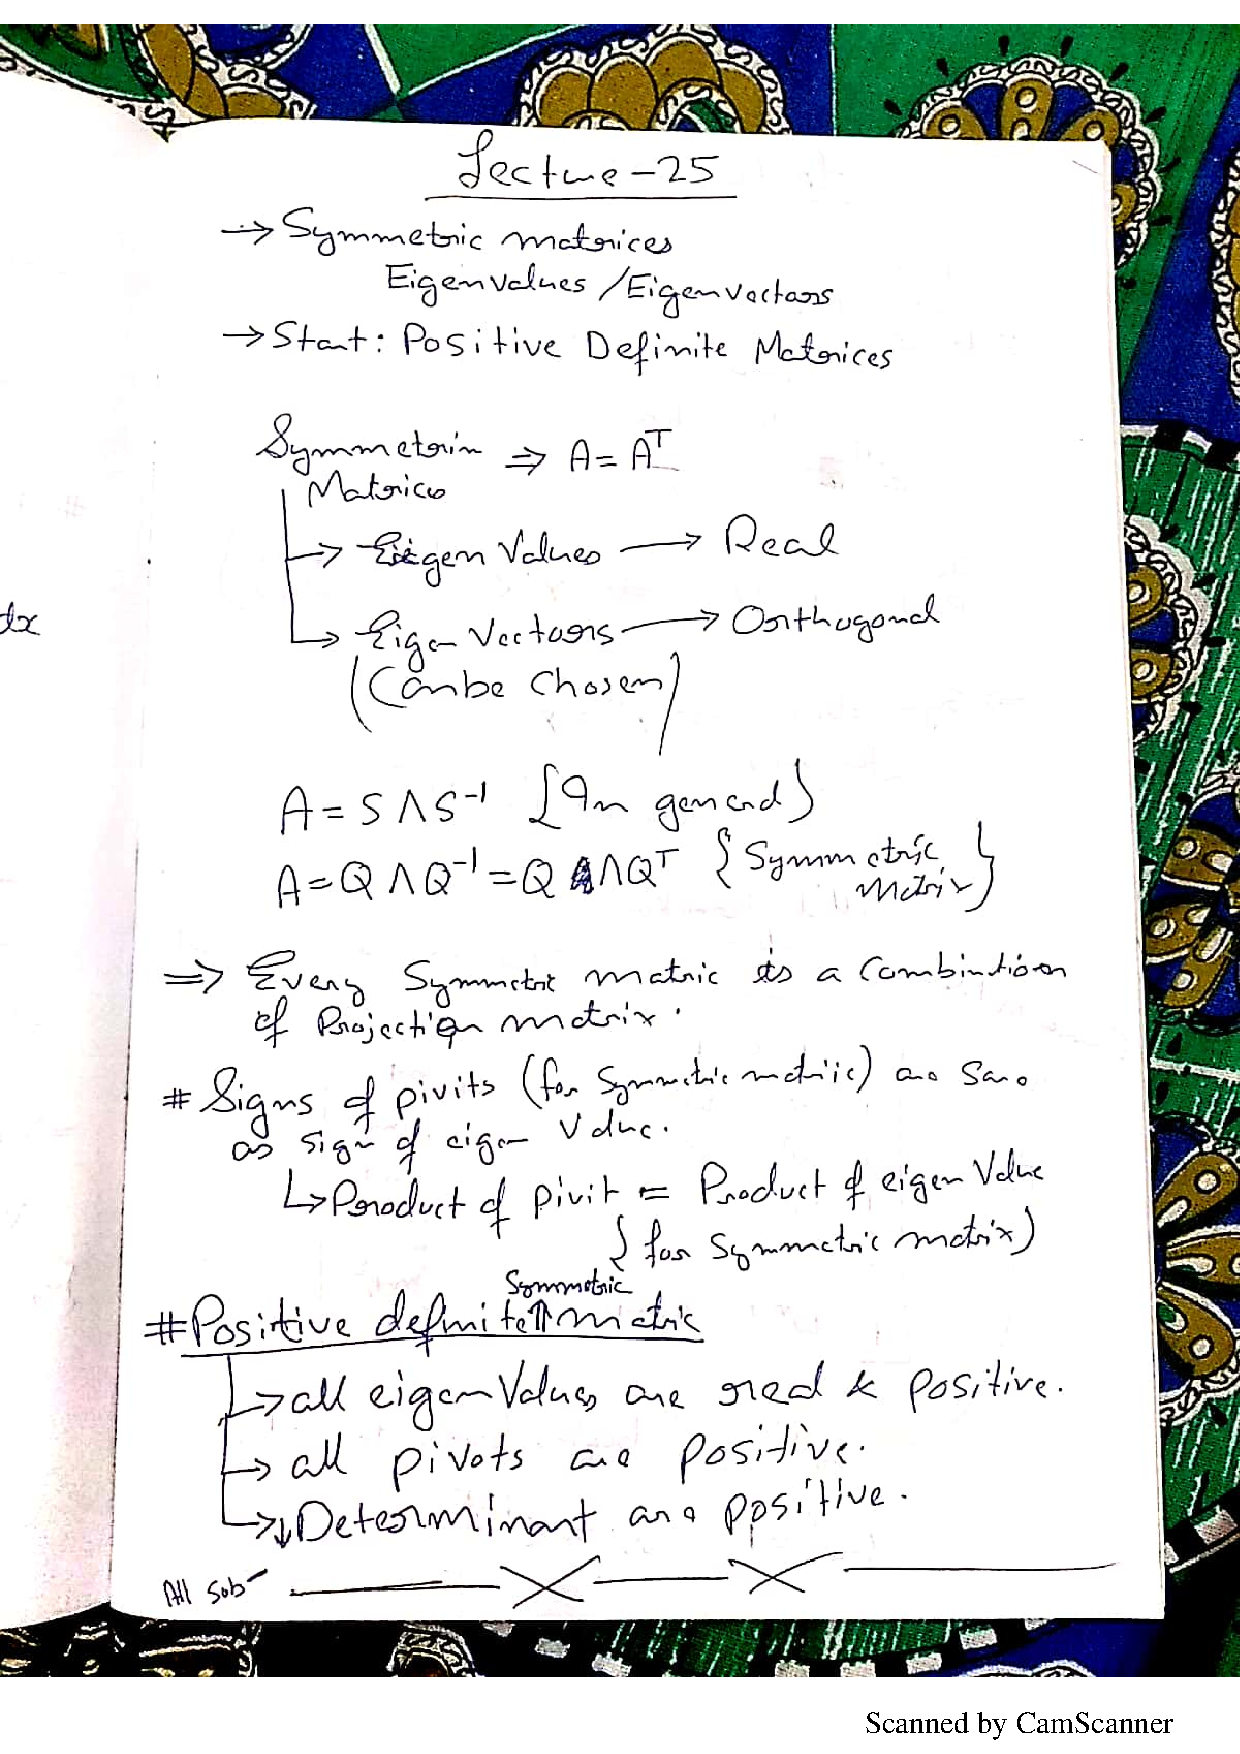
\includepdf[page=-]{./raw_files/25.pdf}

\chapter{Lecture 26}
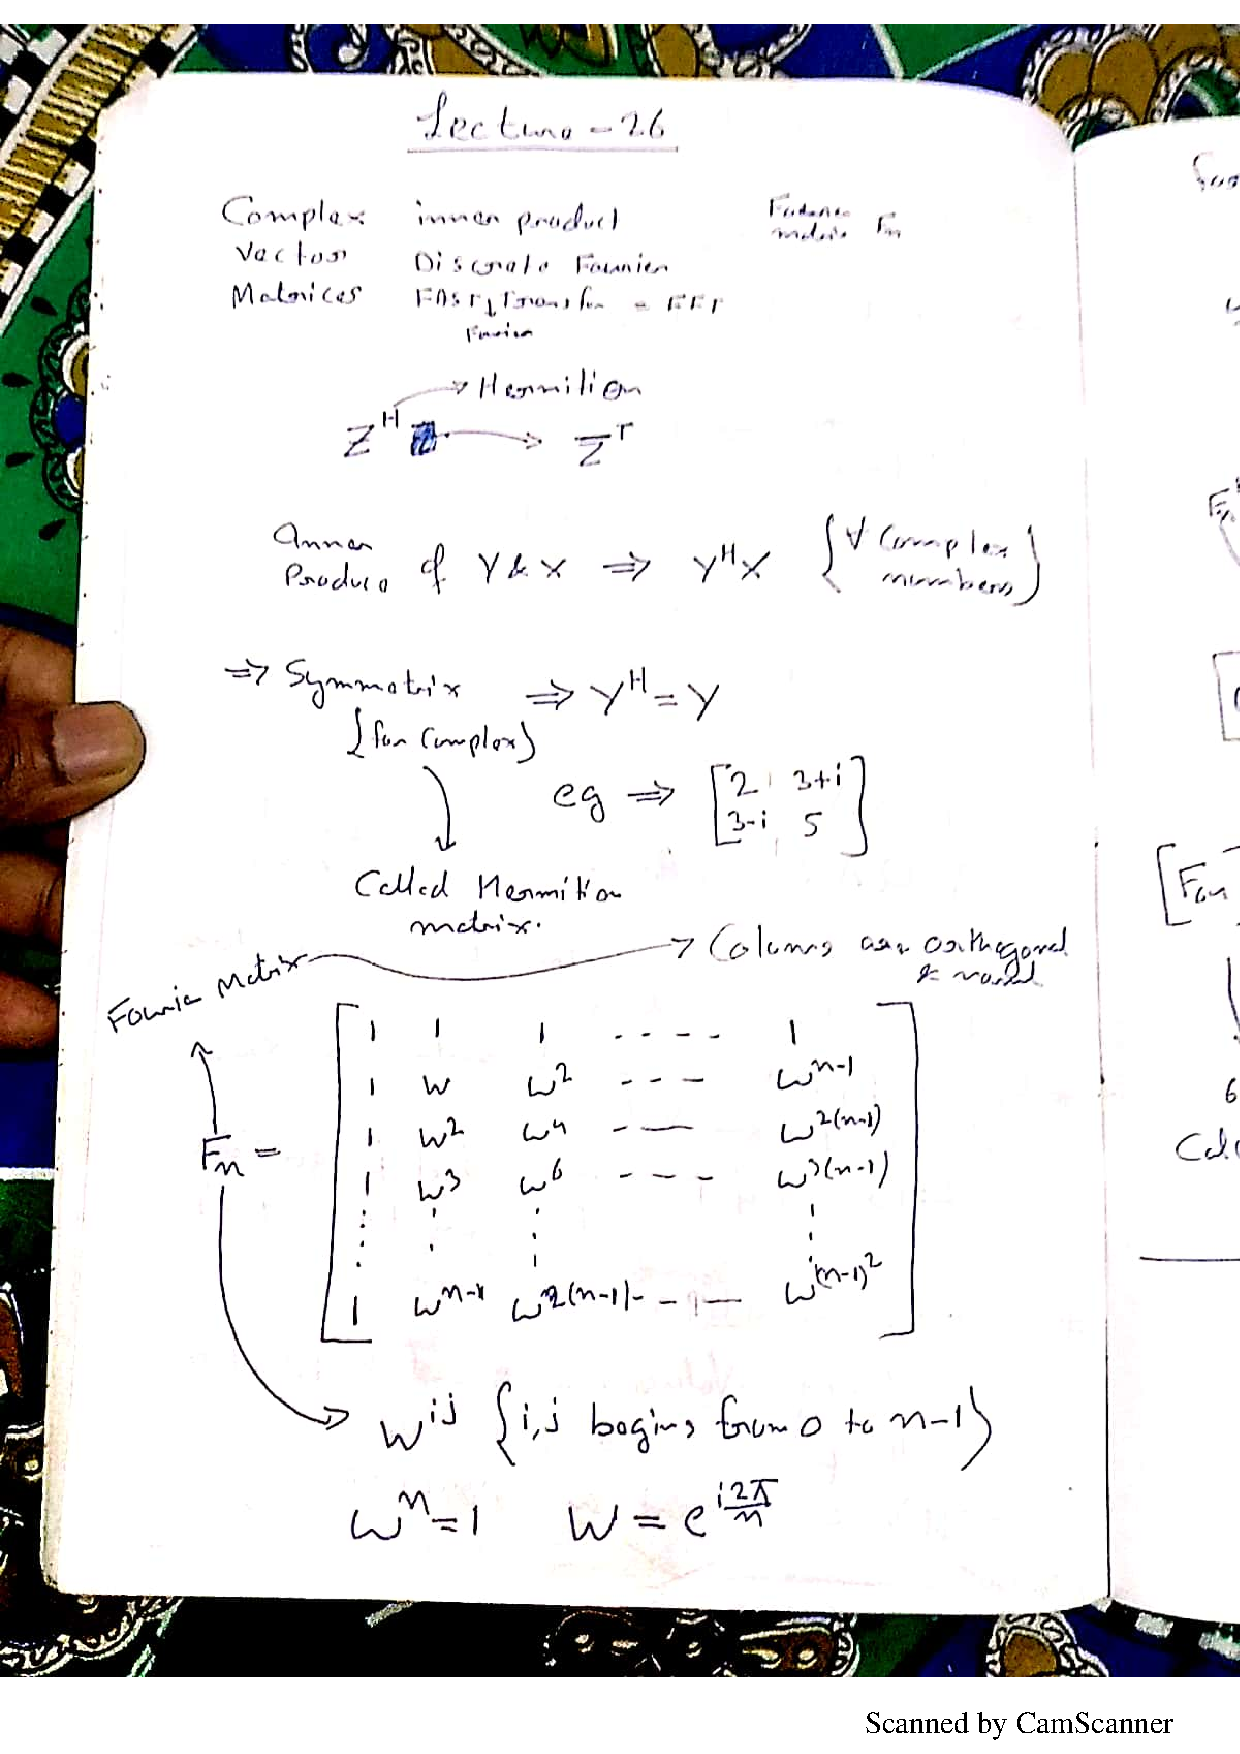
\includepdf[page=-]{./raw_files/26.pdf}

\chapter{Lecture 27}
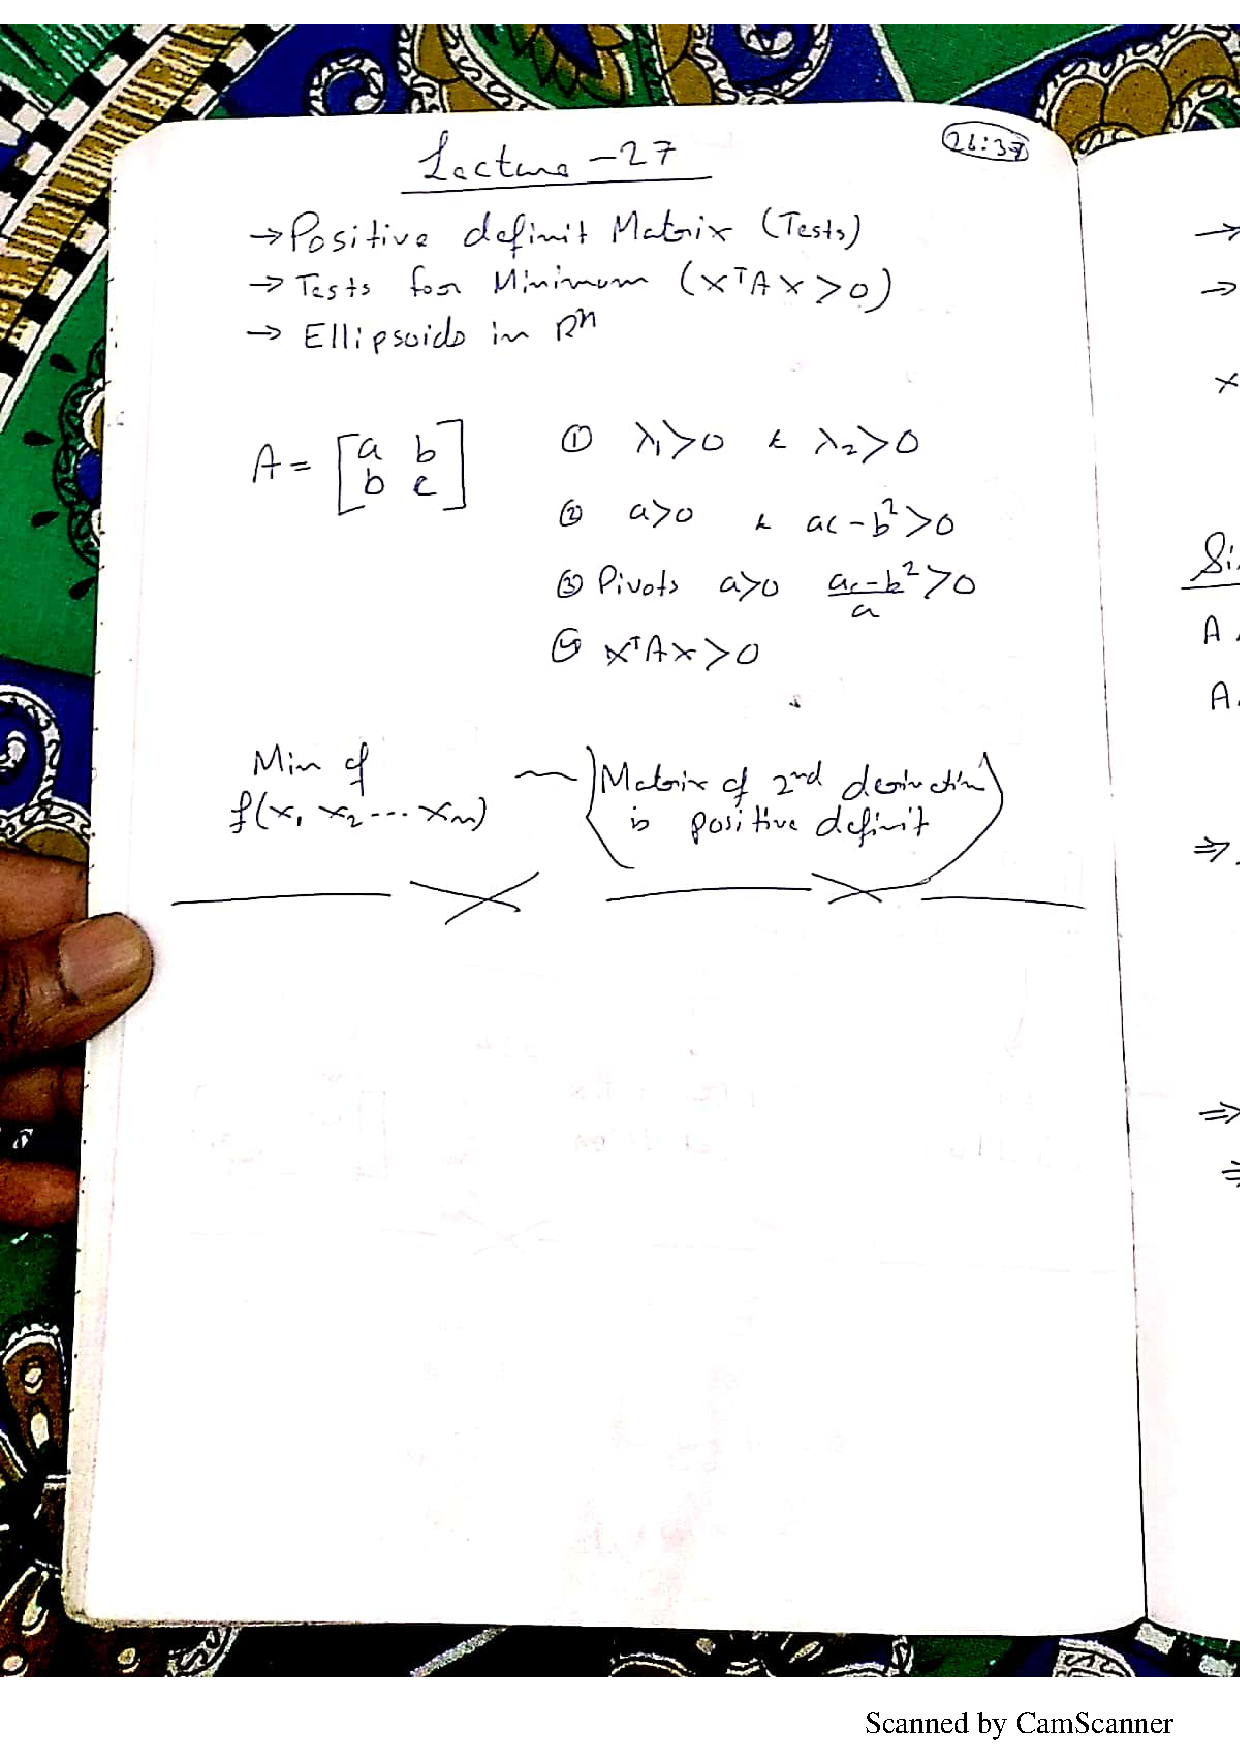
\includepdf[page=-]{./raw_files/27.pdf}

\chapter{Lecture 28}
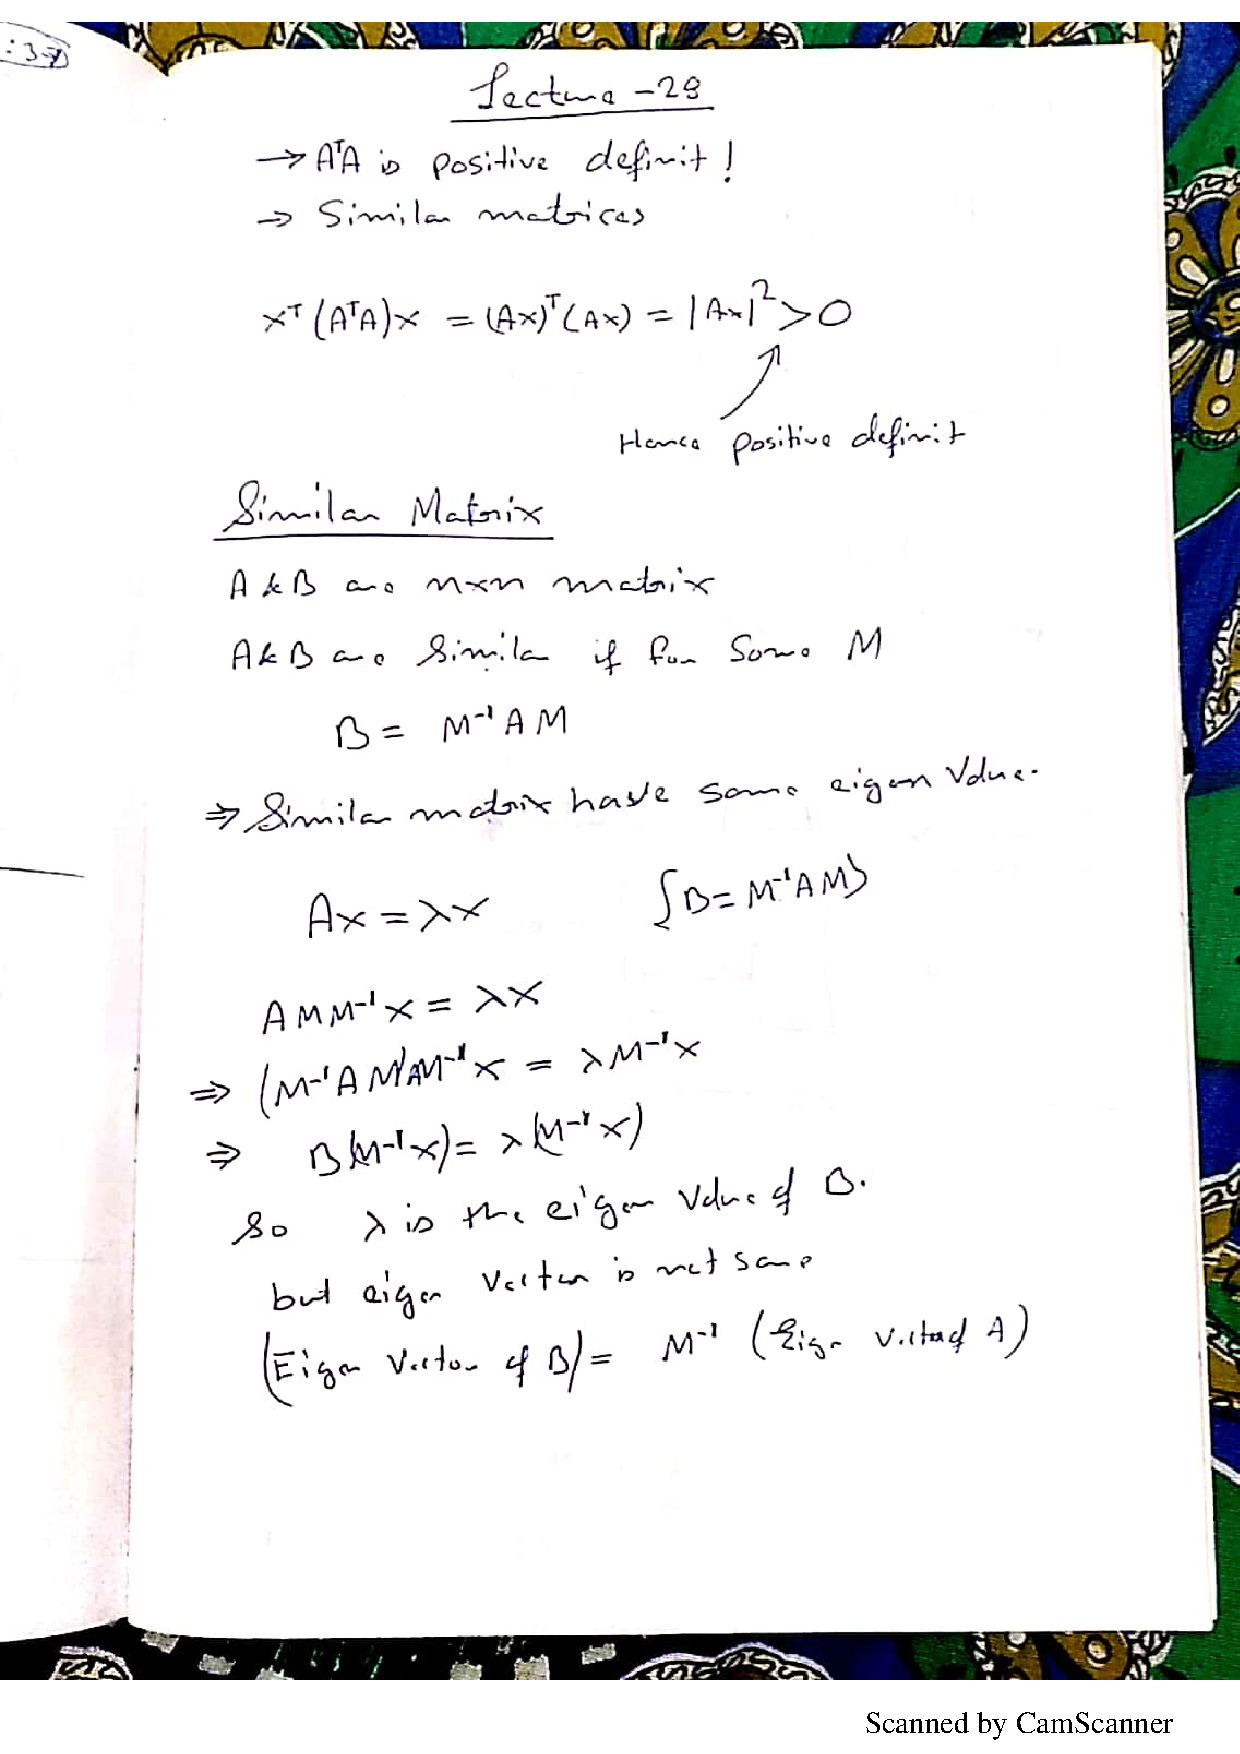
\includepdf[page=-]{./raw_files/28.pdf}

\chapter{Lecture 29}
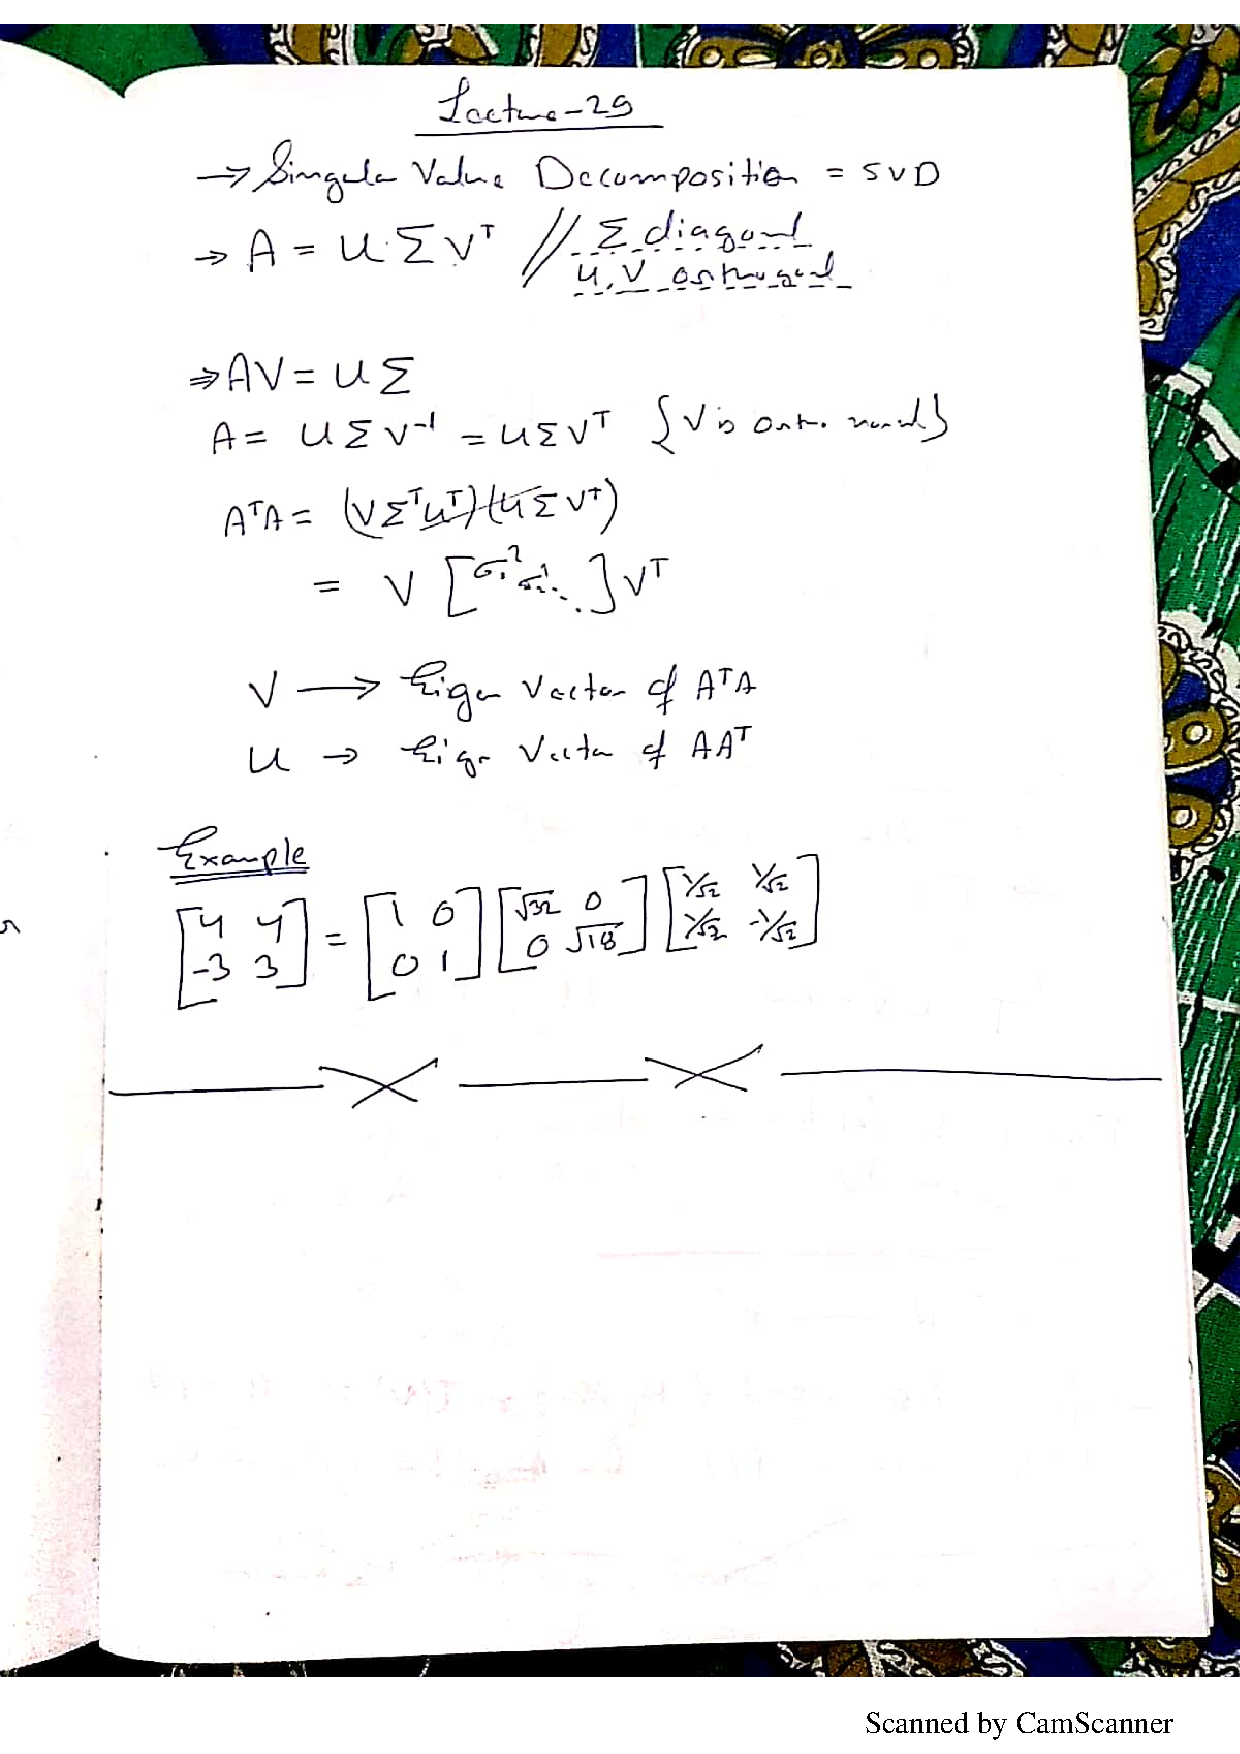
\includepdf[page=-]{./raw_files/29.pdf}

\chapter{Lecture 30}
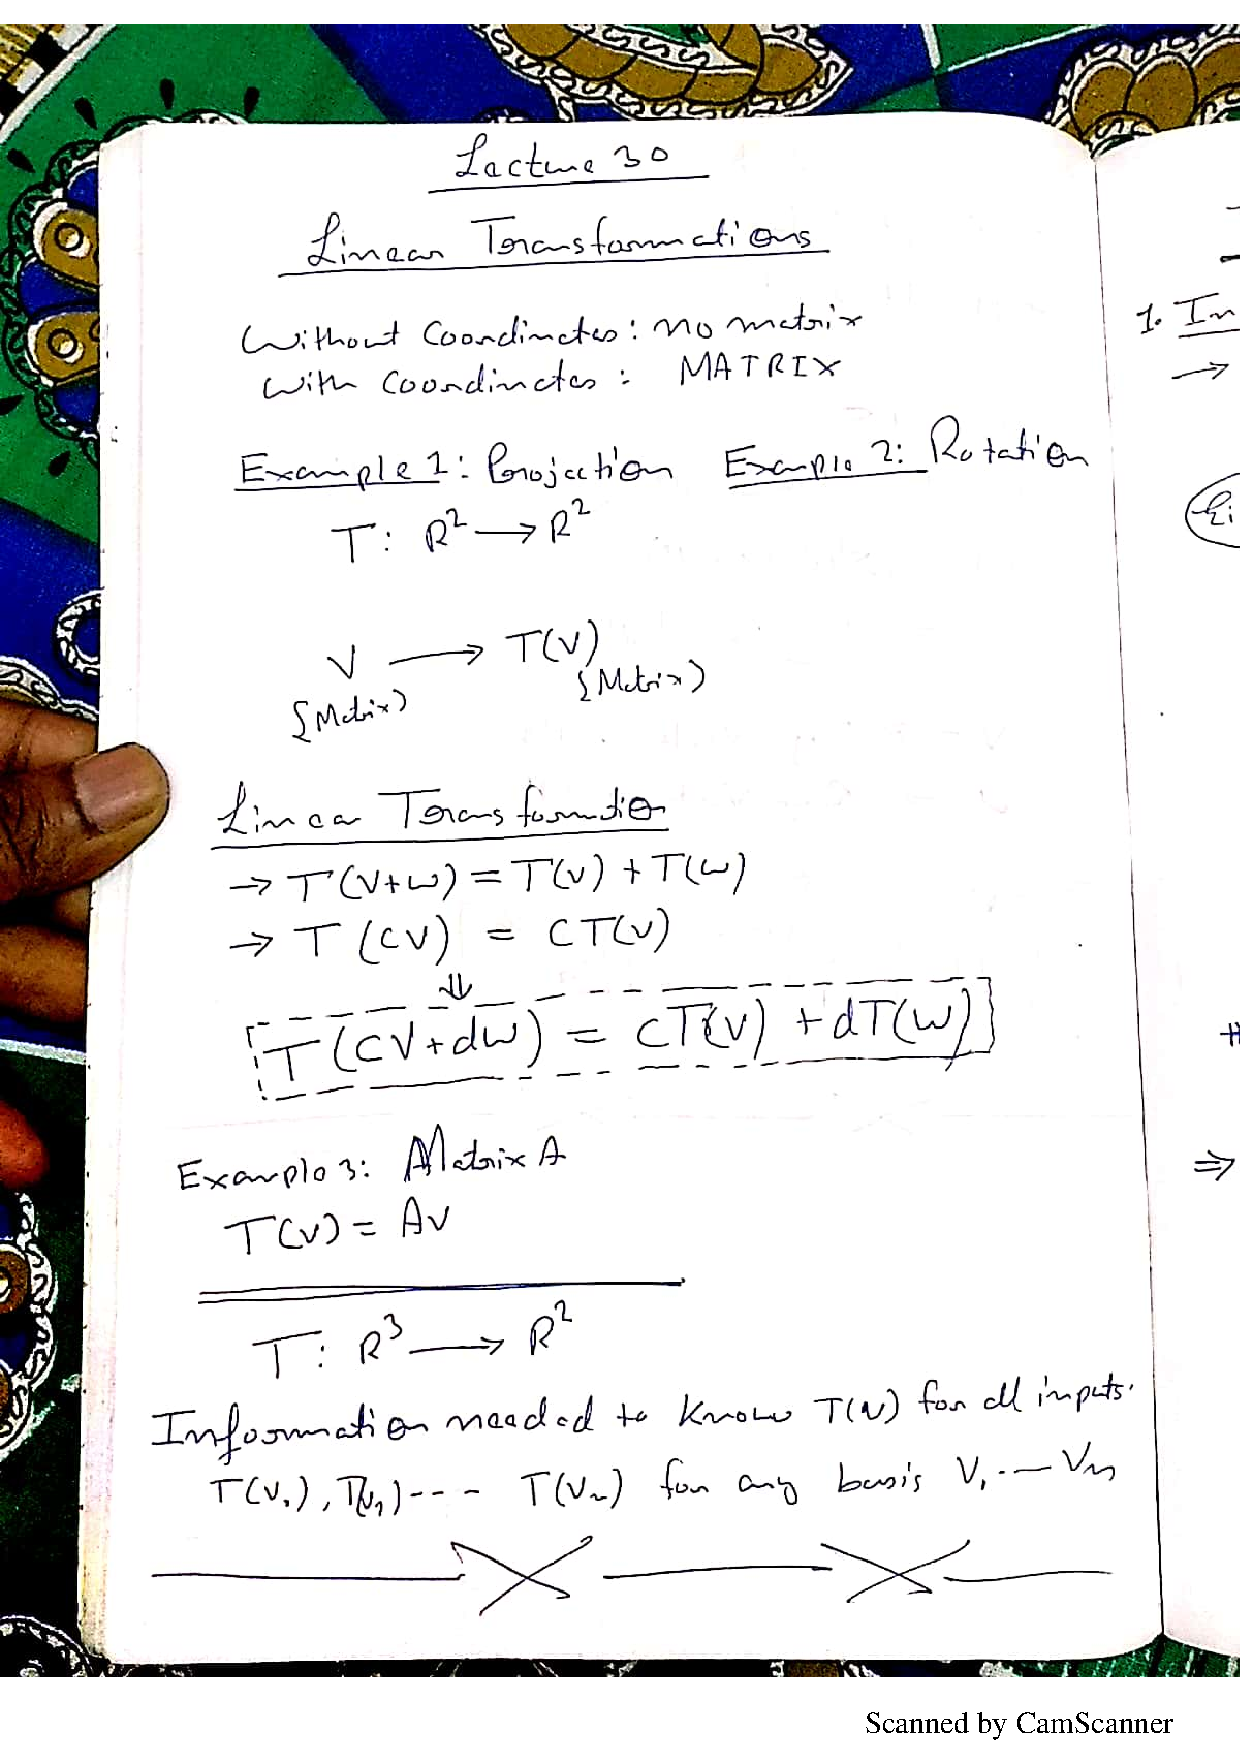
\includepdf[page=-]{./raw_files/30.pdf}

\chapter{Appendix 1}
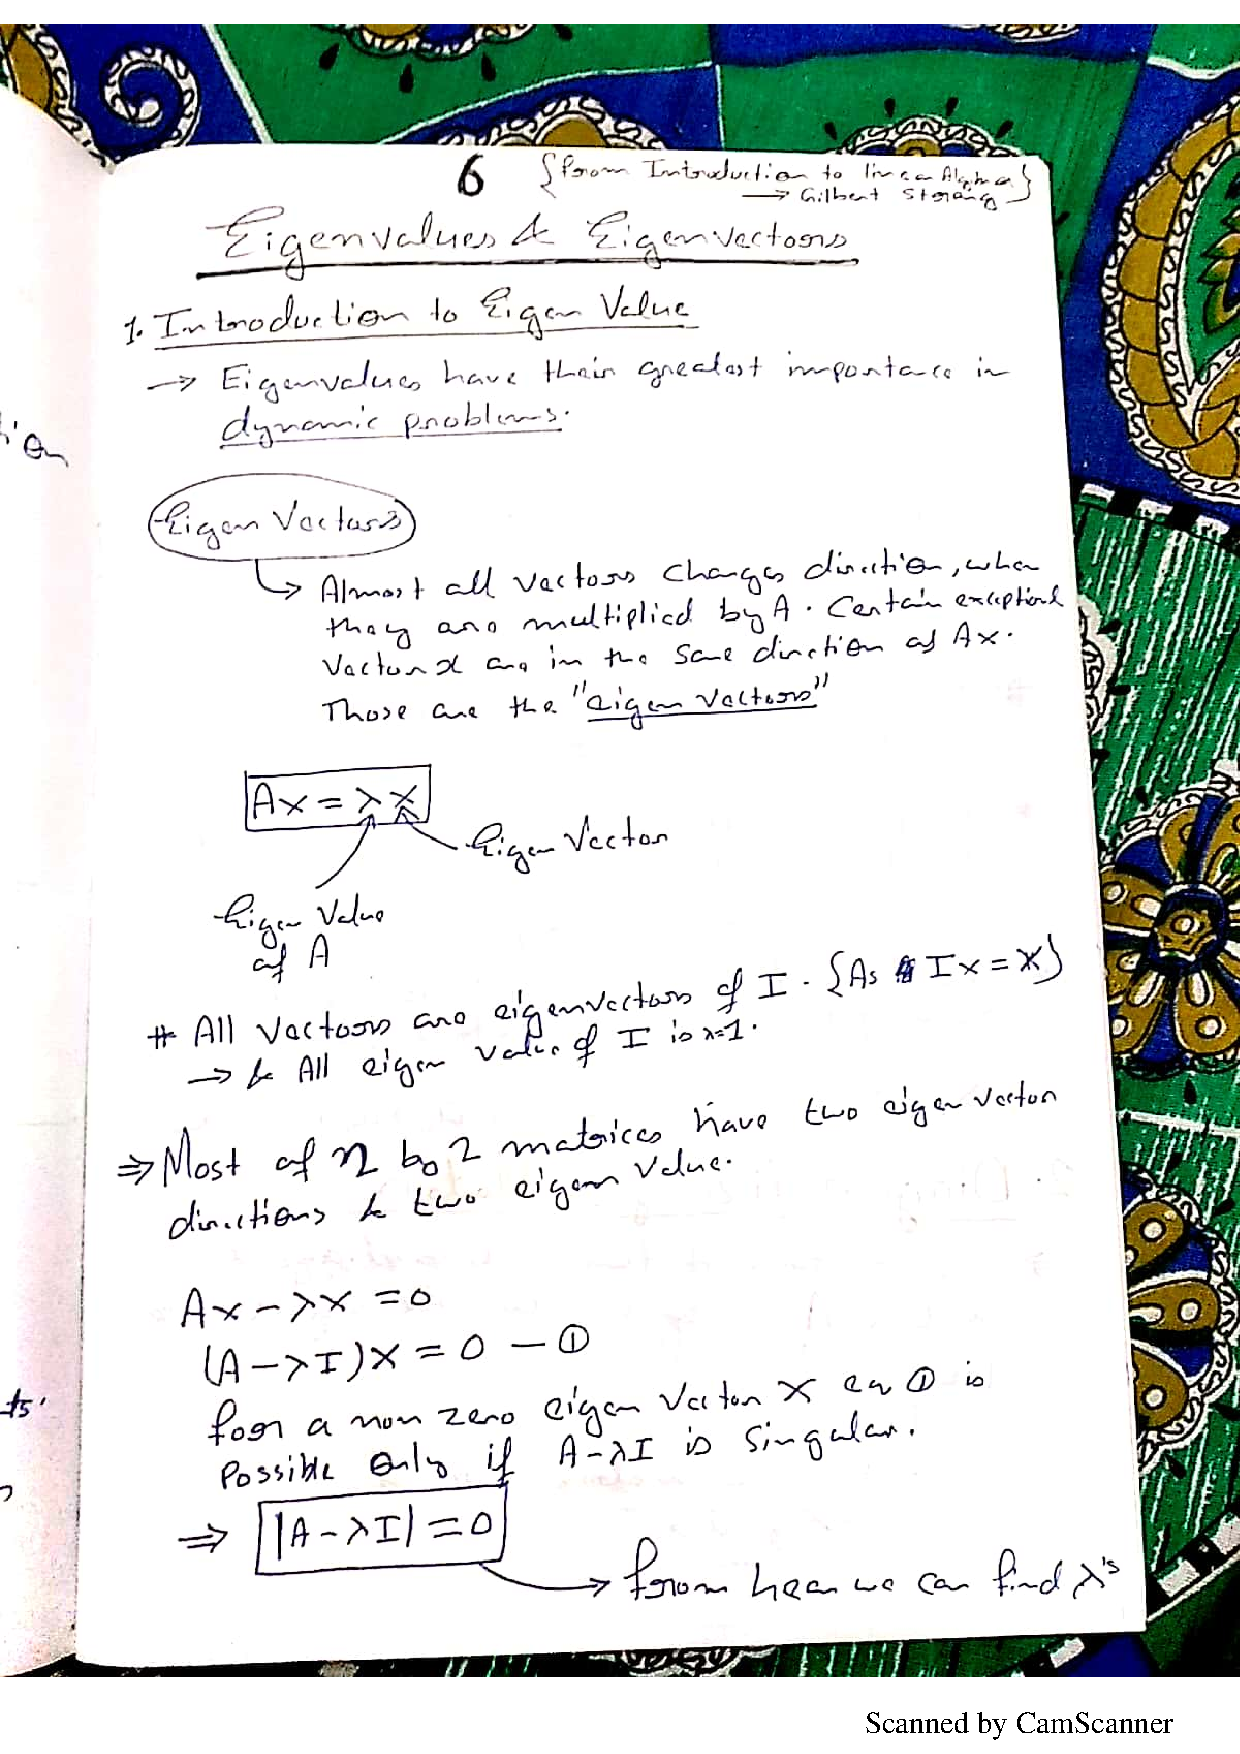
\includepdf[page=-]{./raw_files/a1.pdf}

\chapter{Appendix 2}
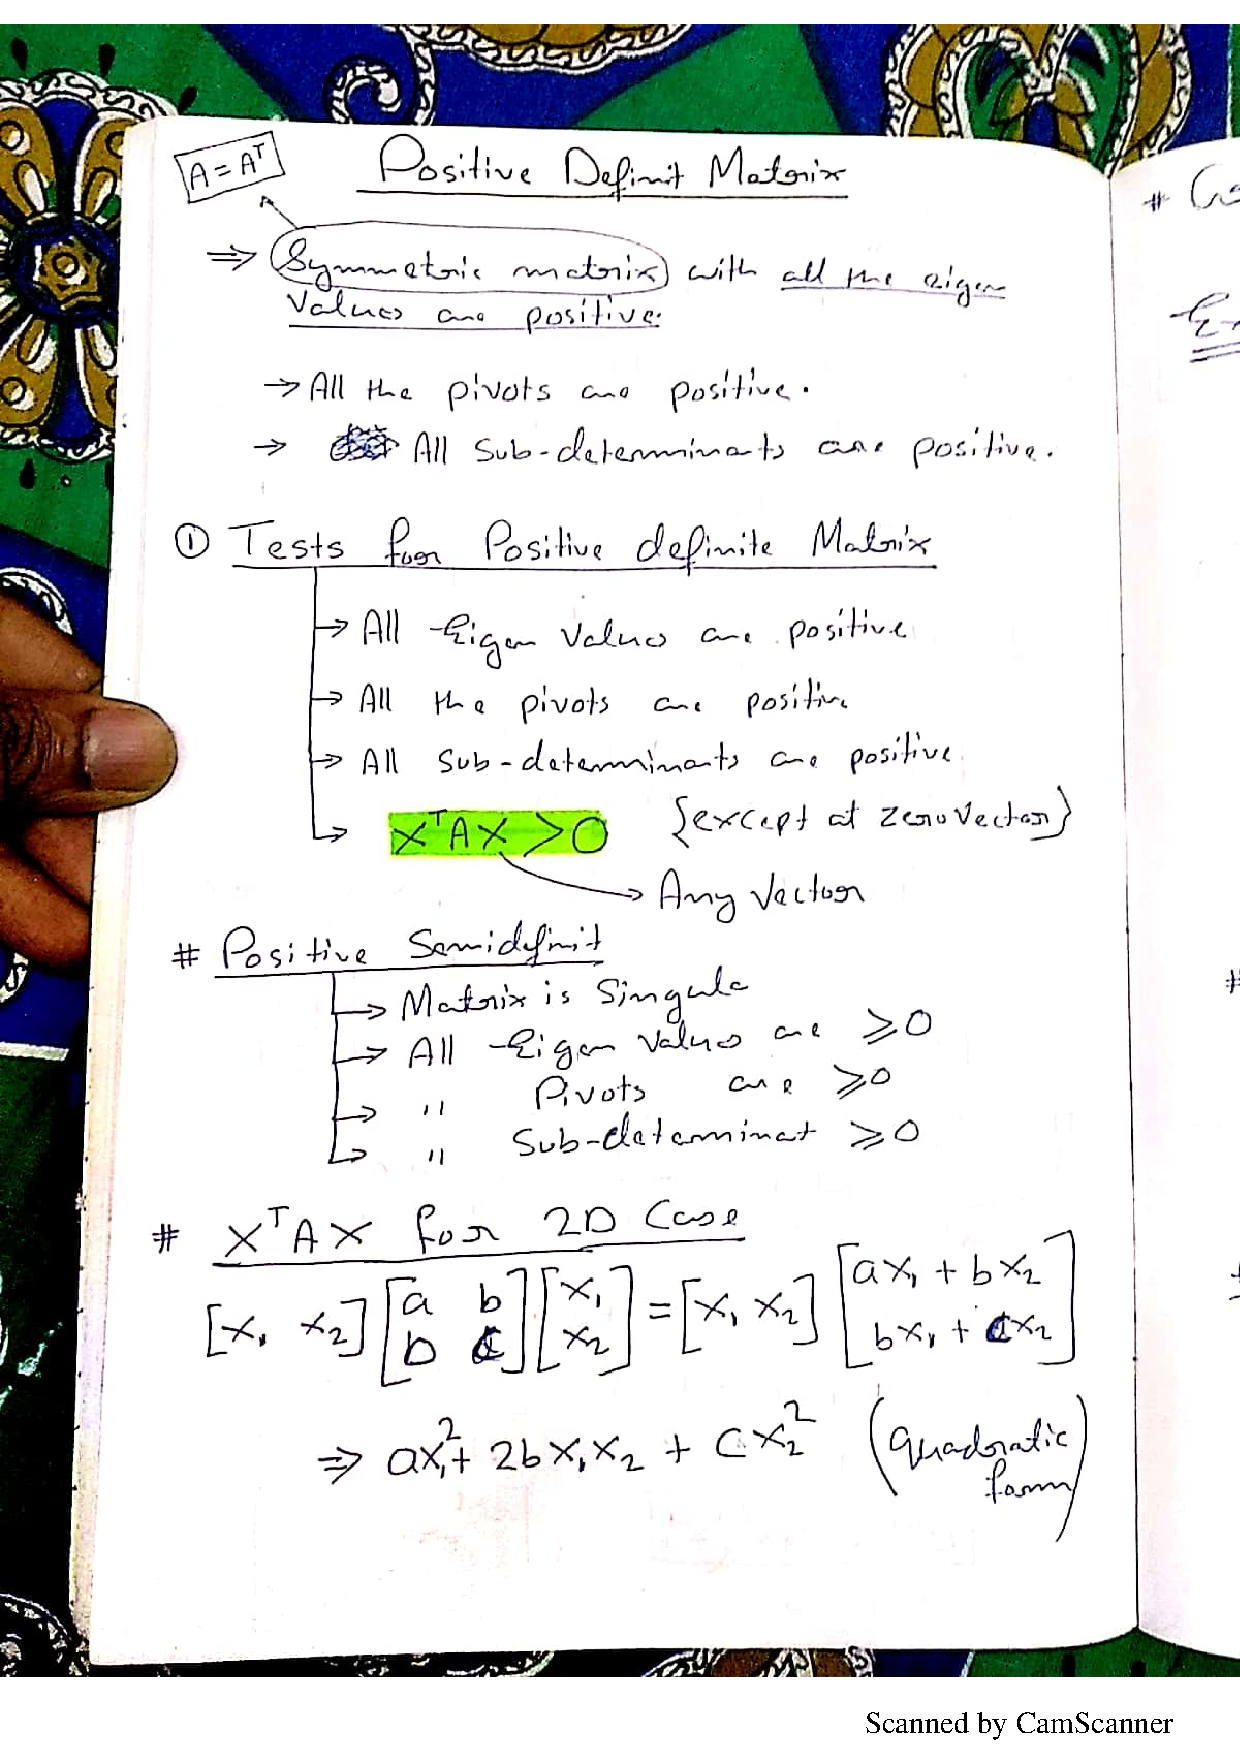
\includepdf[page=-]{./raw_files/a2.pdf}


\end{document}